%" vim: fdm=marker:fen:fdl=0
%%%%%%%%%%%%%%%%%%%%%%%%%%%%%%%%%%%%%%%%%%%%%%%%%%%%
% Document type, global settings, and packages
%%%%%%%%%%%%%%%%%%%%%%%%%%%%%%%%%%%%%%%%%%%%%%%%%%%%

%	Settings and Packages%{{{1
\documentclass[12pt]{report}   %12 point font for Times New Roman
\usepackage{graphicx}  %for images and plots
\usepackage[letterpaper, left=1.5in, right=1in, top=1in, bottom=1in]{geometry}
\graphicspath{{figures/}}
\usepackage{setspace}  %use this package to set linespacing as desired
\usepackage{times}  %set Times New Roman as the font
\usepackage[explicit]{titlesec}  %title control and formatting
\usepackage[titles]{tocloft}  %table of contents control and formatting
\usepackage[backend=bibtex, sorting=none, bibstyle=ieee]{biblatex}  %reference manager
\usepackage[page]{appendix}  %for appendices
\usepackage{rotating}  %for rotated, landscape images
\usepackage{ulem}  %for underlined section titles
\usepackage{siunitx}  %for units
\usepackage{amsmath,amsthm,amssymb,amsfonts} 
\usepackage[bookmarks=true, hidelinks]{hyperref}
%	
%%%%%%%%%%%%%%%%%%%%%%%%%%%%%%%%%%%
% Bibliography
%%%%%%%%%%%%%%%%%%%%%%%%%%%%%%%%%%%

%Add your bibliography file here
\bibliography{references}

% prevent certain fields in references from printing in bibliography
\AtEveryBibitem{\clearfield{issn}}
\AtEveryBibitem{\clearlist{issn}}

\AtEveryBibitem{\clearfield{language}}
\AtEveryBibitem{\clearlist{language}}

\AtEveryBibitem{\clearfield{doi}}
\AtEveryBibitem{\clearlist{doi}}

\AtEveryBibitem{\clearfield{url}}
\AtEveryBibitem{\clearlist{url}}

\AtEveryBibitem{%
  \ifentrytype{online}
    {}
    {\clearfield{urlyear}\clearfield{urlmonth}\clearfield{urlday}}}

%%%%%%%%%%%%%%%%%%%%%%
% Start of Document
%%%%%%%%%%%%%%%%%%%%%%

\begin{document}
\doublespacing  %set line spacing

%%%%%%%%%%%%%%%%%%%%%%%%%%%%%%%%%%%%%
% \input for title page through acknowledgements
%%%%%%%%%%%%%%%%%%%%%%%%%%%%%%%%%%%%%

%input: title, approval, epigraph, dedication, acknowledgments%{{{
%%%%%%%%%%%%%%%%%%%%%%%%%%%%%%%%%%%%%
% Title Page
%%%%%%%%%%%%%%%%%%%%%%%%%%%%%%%%%%%%%

%% Define your thesis title, your name, your school, and your month and year of graduation here

\newcommand{\thesisTitle}{Development of HPGe Detector Systems at The University of South Dakota}
\newcommand{\yourName}{Mitchell D. Wagner}
\newcommand{\yourSchool}{The University of South Dakota}
\newcommand{\yourMonth}{May}
\newcommand{\yourYear}{2018}

%%%%%%%%%%%%%%%%%%%%%%%%%%%%%%%%%%%%%%%%%%%%%%%%%%%%%%%%%
% Do not edit these lines unless you wish to customize
% the template
%%%%%%%%%%%%%%%%%%%%%%%%%%%%%%%%%%%%%%%%%%%%%%%%%%%%%%%%%



\begin{titlepage}
\begin{center}

\begin{singlespacing}

\textbf{\MakeUppercase{\thesisTitle}}\\
\vspace{10\baselineskip}
A Dissertation\\
Presented to\\
The Academic Faculty\\
\vspace{3\baselineskip}
By\\
\vspace{3\baselineskip}
\yourName\\
\vspace{3\baselineskip}
In Partial Fulfillment\\
of the Requirements for the Degree\\
Master of Science in the\\
School of \yourSchool\\
\vspace{3\baselineskip}
The University of South Dakota\\
\vspace{\baselineskip}
\yourMonth{} \yourYear{}
\vfill
Copyright \copyright{} \yourName{} \yourYear{}

\end{singlespacing}

\end{center}
\end{titlepage}



\currentpdfbookmark{Title Page}{titlePage}  %add PDF bookmark for this page

%%%%%%%%%%%%%%%%%%%%%%%%%%%%%%%%%%%%%
% Approval Page
%%%%%%%%%%%%%%%%%%%%%%%%%%%%%%%%%%%%%

%% Define your committee members. If you have less than 6, simple delete/comment the unused lines

\newcommand{\committeeMemberOne}{Dr. Jing Liu, Advisor}
\newcommand{\committeeMemberOneDepartment}{Physics}
\newcommand{\committeeMemberOneAffiliation}{University of South Dakota}

\newcommand{\committeeMemberTwo}{Dr. Dongming Mei}
\newcommand{\committeeMemberTwoDepartment}{Physics}
\newcommand{\committeeMemberTwoAffiliation}{University of South Dakota}

\newcommand{\committeeMemberThree}{Dr. Miles Koppang}
\newcommand{\committeeMemberThreeDepartment}{Chemistry}
\newcommand{\committeeMemberThreeAffiliation}{University of South Dakota}


\newcommand{\approvalDay}{31}
\newcommand{\approvalMonth}{05}
\newcommand{\approvalYear}{2018}

%%%%%%%%%%%%%%%%%%%%%%%%%%%%%%%%%%%%%%%%%%%%%%%%%%%%%%%%%
% Do not edit these lines unless you wish to customize
% the template
%%%%%%%%%%%%%%%%%%%%%%%%%%%%%%%%%%%%%%%%%%%%%%%%%%%%%%%%%


\begin{titlepage}
\begin{singlespacing}
\begin{center}

\textbf{\MakeUppercase{\thesisTitle}}\\
\vspace{10\baselineskip}

\end{center}
\vfill

%Define minipages, depending on how many authors there are
\ifdefined\committeeMemberFour

Approved by:
\vspace{2\baselineskip}		%adjust the number in front of "\baselineskip" for alignment

\begin{minipage}[b]{0.4\textwidth}
	
	\committeeMemberOne\\
	\committeeMemberOneDepartment\\
	\textit{\committeeMemberOneAffiliation}\\
	
	\committeeMemberTwo\\
	\committeeMemberTwoDepartment\\
	\textit{\committeeMemberTwoAffiliation}\\
	
	\committeeMemberThree\\
	\committeeMemberThreeDepartment\\
	\textit{\committeeMemberThreeAffiliation}\\
	
	\vspace{2\baselineskip}		%adjust the number in front of "\baselineskip" for alignment
	
\end{minipage}
\hspace{0.1\textwidth}
\begin{minipage}[b]{0.4\textwidth}
	
	\committeeMemberFour\\
	\committeeMemberFourDepartment\\
	\textit{\committeeMemberFourAffiliation}\\
	
	\ifdefined\committeeMemberSix
	\committeeMemberFive\\
	\committeeMemberFiveDepartment\\
	\textit{\committeeMemberFiveAffiliation}\\
	
	\committeeMemberSix\\
	\committeeMemberSixDepartment\\
	\textit{\committeeMemberSixAffiliation}\\
	
	Date Approved: \approvalMonth{} \approvalDay, \approvalYear
	\vspace{1\baselineskip}		%adjust the number in front of "\baselineskip" for alignment
	
	\else
	
	\committeeMemberFive\\
	\committeeMemberFiveDepartment\\
	\textit{\committeeMemberFiveAffiliation}\\
		
	Date Approved: \approvalMonth{} \approvalDay, \approvalYear
	\vspace{5\baselineskip}		%adjust the number in front of "\baselineskip" for alignment
	
	\fi
	
\end{minipage}

\else

\hspace{0.6\textwidth}
\begin{minipage}[b]{0.4\textwidth}
	
	Approved by:
	\vspace{2\baselineskip}		%adjust the number in front of "\baselineskip" for alignment
	
	\committeeMemberOne\\
	\committeeMemberOneDepartment\\
	\textit{\committeeMemberOneAffiliation}\\
	
	\committeeMemberTwo\\
	\committeeMemberTwoDepartment\\
	\textit{\committeeMemberTwoAffiliation}\\
	
	\committeeMemberThree\\
	\committeeMemberThreeDepartment\\
	\textit{\committeeMemberThreeAffiliation}\\
	
	\vspace{2\baselineskip}		%adjust the number in front of "\baselineskip" for alignment
	
	Date Approved: \approvalMonth{} \approvalDay, \approvalYear
	\vspace{\baselineskip}		%adjust the number in front of "\baselineskip" for alignment
	
\end{minipage}

\fi





\end{singlespacing}
\end{titlepage}


%%%%%%%%%%%%%%%%%%%%%%%%%%%%%%%%%%%%%
% Epigraph
%%%%%%%%%%%%%%%%%%%%%%%%%%%%%%%%%%%%%

% Define your quote and author for the epigraph here

\newcommand{\yourQuote}{A great quote to start the thesis}
\newcommand{\yourAuthor}{George P. Burdell}

%%%%%%%%%%%%%%%%%%%%%%%%%%%%%%%%%%%%%%%%%%%%%%%%%%%%%%%%%
% Do not edit these lines unless you wish to customize
% the template
%%%%%%%%%%%%%%%%%%%%%%%%%%%%%%%%%%%%%%%%%%%%%%%%%%%%%%%%%

\begin{titlepage}
\begin{center}

\vspace*{\fill}
\yourQuote\\
\textit{\yourAuthor}
\vspace*{\fill}

\end{center}
\end{titlepage}



%%%%%%%%%%%%%%%%%%%%%%%%%%%%%%%%%%%%%
% Dedication
%%%%%%%%%%%%%%%%%%%%%%%%%%%%%%%%%%%%%

% Define your dedication statement here

\newcommand{\yourDedication}{This thesis is dedicated to my family, whose continued support has kept me going.}

%%%%%%%%%%%%%%%%%%%%%%%%%%%%%%%%%%%%%%%%%%%%%%%%%%%%%%%%%
% Do not edit these lines unless you wish to customize
% the template
%%%%%%%%%%%%%%%%%%%%%%%%%%%%%%%%%%%%%%%%%%%%%%%%%%%%%%%%%

\begin{titlepage}
\begin{center}

\vspace*{\fill}
\yourDedication\\
\vspace*{\fill}

\end{center}
\end{titlepage}


%%%%%%%%%%%%%%%%%%%%%%%%%%%%%%%%%%%%%
% Acknowledgments
%%%%%%%%%%%%%%%%%%%%%%%%%%%%%%%%%%%%%

\pagenumbering{roman}
\addcontentsline{toc}{chapter}{Acknowledgments}
\setcounter{page}{6} % set the page number appropriately based on the number of intro pages
\clearpage
\begin{centering}
\textbf{ACKNOWLEDGEMENTS}\\
\vspace{\baselineskip}
\end{centering}

%Insert your dedication text here
The work and research done in this thesis was made possible through the help of my many great professors, advisor, fellow students, and friends.

First and formost I would like to thank my advisor, Dr. Jing Liu, for his continued support, patience, motivation, and life advice, without which I would not have finished my degree

...
\clearpage
%\pagenumbering{gobble}  %remove page number on summary page


%\addtocontents{toc}{\cftpagenumbersoff{chapter}} 

%\currentpdfbookmark{Acknowledgments}{acknowledgments}
%\addtocontents{toc}{\cftpagenumberson{chapter}} %}}}

%%%%%%%%%%%%%%%%%%%%%%%%%%%%%%%%%%%%%
% Table of Contents
%%%%%%%%%%%%%%%%%%%%%%%%%%%%%%%%%%%%%

% Format for Table of Contents%{{{
\renewcommand{\cftchapdotsep}{\cftdotsep}  %add dot separators
\renewcommand{\cftchapfont}{\bfseries}  %set title font weight
\renewcommand{\cftchappagefont}{}  %set page number font weight
\renewcommand{\cftchappresnum}{Chapter }
\renewcommand{\cftchapaftersnum}{:}
\renewcommand{\cftchapnumwidth}{5em}
\renewcommand{\cftchapafterpnum}{\vskip\baselineskip} %set correct spacing for entries in single space environment
\renewcommand{\cftsecafterpnum}{\vskip\baselineskip}  %set correct spacing for entries in single space environment
\renewcommand{\cftsubsecafterpnum}{\vskip\baselineskip} %set correct spacing for entries in single space environment
\renewcommand{\cftsubsubsecafterpnum}{\vskip\baselineskip} %set correct spacing for entries in single space environment%}}}

%format title font size and position (this also applys to list of figures and list of tables)%{{{
\titleformat{\chapter}[display]
{\normalfont\bfseries\filcenter}{\chaptertitlename\ \thechapter}{0pt}{\MakeUppercase{#1}}

\renewcommand\contentsname{Table of Contents}

\begin{singlespace}
\tableofcontents
\end{singlespace}

\currentpdfbookmark{Table of Contents}{TOC}

\clearpage%}}}

%%%%%%%%%%%%%%%%%%%%%%%%%%%%%%%%%%%%%
% List of figures and tables
%%%%%%%%%%%%%%%%%%%%%%%%%%%%%%%%%%%%%

%figures and tables formating%{{{
\addcontentsline{toc}{chapter}{List of Tables}
\begin{singlespace}
	\setlength\cftbeforetabskip{\baselineskip}  %manually set spacing between entries
	\listoftables
\end{singlespace}

\clearpage

\addcontentsline{toc}{chapter}{List of Figures}
\begin{singlespace}
\setlength\cftbeforefigskip{\baselineskip}  %manually set spacing between entries
\listoffigures
\end{singlespace}

\clearpage
%}}}

%%%%%%%%%%%%%%%%%%%%%%%%%%%%%%%%%%%%%%%%%%%%%%%%%%%%%%%%%%%%%%%%%
% This is the Summary (abstract should be separate document)
%%%%%%%%%%%%%%%%%%%%%%%%%%%%%%%%%%%%%%%%%%%%%%%%%%%%%%%%%%%%%%%%%

\clearpage
\begin{centering}
\textbf{SUMMARY}\\
\vspace{\baselineskip}
\end{centering}

Lorem ipsum dolor sit amet, consectetur adipiscing elit, sed do eiusmod tempor incididunt ut labore et dolore magna aliqua. Ut enim ad minim veniam, quis nostrud exercitation ullamco laboris nisi ut aliquip ex ea commodo consequat. Duis aute irure dolor in reprehenderit in voluptate velit esse cillum dolore eu fugiat nulla pariatur. Excepteur sint occaecat cupidatat non proident, sunt in culpa qui officia deserunt mollit anim id est laborum.

%\pagenumbering{gobble}  %remove page number on summary page

%%%%%%%%%%%%%%%%%%%%%%%%%%%%
%
% Chapters
%
%%%%%%%%%%%%%%%%%%%%%%%%%%%%

%%%%%%%%%%%%%%%%%%%%%%
% formatting%{{{

% resume page numbering for rest of document
\clearpage
\pagenumbering{arabic}
\setcounter{page}{1} % set the page number appropriately

% Adjust chapter title formatting
\titleformat{\chapter}[display]
{\normalfont\bfseries\filcenter}{\MakeUppercase\chaptertitlename\ \thechapter}{0pt}{\MakeUppercase{#1}}  %spacing between titles
\titlespacing*{\chapter}
  {0pt}{0pt}{30pt}	%controls vertical margins on title
  
% Adjust section title formatting
\titleformat{\section}{\normalfont\bfseries}{\thesection}{1em}{#1}

% Adjust subsection title formatting
\titleformat{\subsection}{\normalfont}{\uline{\thesubsection}}{0em}{\uline{\hspace{1em}#1}}

% Adjust subsubsection title formatting
\titleformat{\subsubsection}{\normalfont\itshape}{\thesubsection}{1em}{#1}
%}}}
%%%%%%%%%%%%%%%%%%%%%%

%%%%%%%%%%%%%%%%%%%%%%
%input chapters1-7, appendices%{{{
%%%%%%%%%%%%%%%%
% Chapter 1
%%%%%%%%%%%%%%%%

\chapter{Introduction and Background}

Since birth, the Earth has been under a constant barrage of particles.
Some can be seen with the naked eye, such as a portion of the light from the sun and stars, while others such as x-rays or microwaves cannot.
The discovery of radioactivity by Henri Becquerel in 1896 when he was studying phosporescence \cite{Mould} coupled with Wilhelm R{\"o}ntgen's discovery of x-rays in 1895 \cite{wilhelm} kickstarted the search for devices capable of detecting these invisible particles.

One of the early and most widely used radiation detection device was the Geiger-M{\"u}ller tube developed in 1928 \cite{geiger}.
The device utalized a tube filled with gas coupled to a power supply and some simple electronics and was able to see several different types of ionizing radiation.
However, the drawback is that it was only able to count particles and could not give any information about the energy or type of particle observed.
Development of new radiation detectors continued in an effort to be able to precisly measure the energy carried by different types of energy and better understand their interactions with matter.
The 1950s and 60s saw the development of a new type of device called a semiconductor diode detector with the two types of material most widely used being Silicon and Germanium.
This thesis will focus on the development of germanium detectors

The initial development of germanium detectors came a few years after the concept was demonstrated using silicon.
The first working detector used a lithium drifted contact and was created in 1962 by D. V. Freck and J. Wakefield \cite{1962Natur}
How precisly these first developed detectors could measure the energy was, however, something to be desired.
They were held back by the limitations of purifying the germanium and the speed of the electronics.
This put germanium detectors on ice until further development led to the creation of high purity germanium (HPGe) detectors in 1970 \cite{Baertsch1970,Tavendale1970}.

New detectors made from HPGe were able to measure particle energy with almost 10 times betters accuracy which pushed them to be the most sensitive detectors yet created.
Since the 1970s, HPGe detector technology has been advancing rapidly along with the electronics required to make them useable.
The modern era has seen HPGE detetors used in space exploration, medicine, homeland security, natural sciences and now for the next generation of physics experiments.

HPGe detectors have been a standard in the scientific industry for the last 40 years due to their precision and accuracy measuring certain types of radiation in material assay.
More recently, National labs and companies have been producing specialized detectors for multiple cutting edge experiments in the areas of nuclear and astroparticle physics, astronomy, and the search for physics beyond the standard model.
Germanium detectors are becoming a standard tool for a broad spectrum of uses in the next generation of physics experiments and will remain on the forefront for years to come.

nuclear physics \cite{gretina} \cite{agata}

astronomy \cite{astronomy}

dark matter 
CDEX \cite{cdex}
COGENT \cite{cogent}

neutrino physics
Majorana \cite{majorana}
GERDA \cite{gerda}
COHERENT \cite{coherent}


Radioactive material such as uranium has seen use in the energy sector in the form of fuel for nuclear reactors and also in the weapons sector as the payload of nuclear bombs.
It can be dangerous material if handled improperly and in the past has led to mass destruction of cities and ecological zones.
Thankfully, dangerous materials like uranium and polonium can be uniquely identified by the radiation they give off.
Germanium detectors have the ability to detect and identify these elements and can even determine the quantity and direction they are in.
This is what makes HPGe detectors useful to government organizations like the Department of Homeland Security in the United States.
Portable devices are in service all around the US at ports and border crossings to search for the import and export of dangerous material with development ongoing at places like the Pacific Northwest National Laboratory \cite{StaveHS}.

Several applications of HPGe are also seen in the field of nuclear medicine.
Radiopharmaceuticals are dosed to a patient who can then be imaged using an external detector.
For example, single-photon emission computed tomography (SPECT) is a technique to image the gamma rays emitted by injected radiopharmaceuticals.
HPGe detectors have been succesfully demonstrated to have potential in small animal SPECT \cite{SPECT} and also with use in PET scanners.



%%%%%%%%%%%%%%%%
% Chapter 2
%%%%%%%%%%%%%%%%

\chapter{Working Principles of Germanium Detectors}


\section{Mechanical Processing}

This is a section in Chapter 2.


\subsection{Example Subsection}

This is a subsection in Chapter 2.

\subsubsection{Example Subsubsection}

This is a subsubsection in Chapter 2.

% This is a figure in landscape orientation
\begin{sidewaysfigure}
\includegraphics[width=\textwidth]{figures/sput-flow}
\caption{This is another example Figure, rotated to landscape orientation.}
\label{LandscapeFigure}
\end{sidewaysfigure}


%%%%%%%%%%%%%%%%
% Chapter 3
%%%%%%%%%%%%%%%%

\chapter{Principles of Germanium Detectors}
The phase of the detector medium plays an important role in radiation detection.
Gases, liquids, and solids are often used in scintillation detectors and can have huge detector volumes.
However, as shown above, some radiation can pass through these detectors due to gas and liquids having a low density and radiation such as gamma rays being quite penetrating.
Solids can be hundreds or thousands times more dense than gas and thus can have smaller detector volume to detect equivalent energy.
The problem is that even solid scintillation counters have poor energy resolution due to the small number of information carriers.
This is due to the fact that and incoming particle must go from radiation to light to electric signal which has extra steps where data can be lost and statistical fluctuations on small numbers create a limit to the energy resolution.
In order to reduce the statistical limit it is necessary to increase the number of information carriers.
Semiconductor detectors provide increased energy resolution due to more information carriers in terms of electron-hole pairs where the motion of these pairs in an applied electric field generates the electric signal.
Other advantages of semi conductor detectors are: compact size, relatively fast timing characteristics, and variable effective thickness based on application.
The two types of semiconductors most widely used are silicon and germanium.
Silicon is used primarily for charged particle spectroscopy while germanium is more widely used in gamma-ray spectroscopy.

\section{semiconductor diode detectors} 

The band structure of semiconductors is what makes them useful as radiation detectors in comparison to other metals or insulators
In a semiconductor, the valence band is made up of the electrons in the outer shell which are bound to specific lattice sites in the crystal.
In germanium they are covalent bonds that make up the interatomic forces within the crystal.
Above the valence band in terms of energy is the conduction band.
\begin{figure}[htpb]
\centering
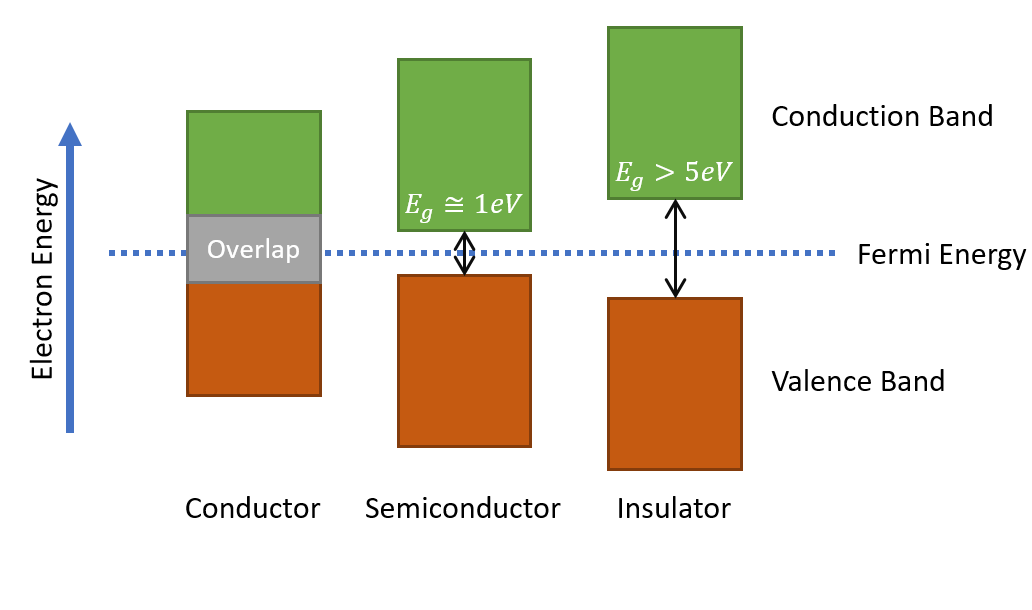
\includegraphics[width=0.9\textwidth]{bandgap}
\caption{Bandgap structures for different material types}
\label{fig:bandgap}
\end{figure}
The conduction and valence bands are separated by a bandgap which is specific to the material type.
The number of electrons inside the crystal just fills the valence band.
If the bandgap is small enough, electrons can sometimes have enough thermal energy to jump to the conduction band.
This energy comes from the crystal and electrons sharing thermal energy at temperatures above absolute zero.
The electron moving to the conduction band leaves behind an empty spot in the valence band which is called a hole.
If an electric field is applied to the crystal, the electron in the conduction band will drift parallel to the field in the opposite direction.
The hole is also acted upon by the field and will be forced to drift in the direction of the field.

All materials have some impurities that affect the crystal structure and can take the place of germanium atoms.
Some of them have electrons in the outer shells that exceed the amount required by the crystal lattice (4) and are thus weakly bonded.
It will not leave a hole behind when it is moved to the conduction band.
Impurities of this type are called donor impurities.
If a material is doped with atoms that have less electrons than required by the lattice, such as those from group III of the periodic table, there will be an extra hole available to be filled.  This is called an acceptor site.
\begin{figure}[htpb]
\centering
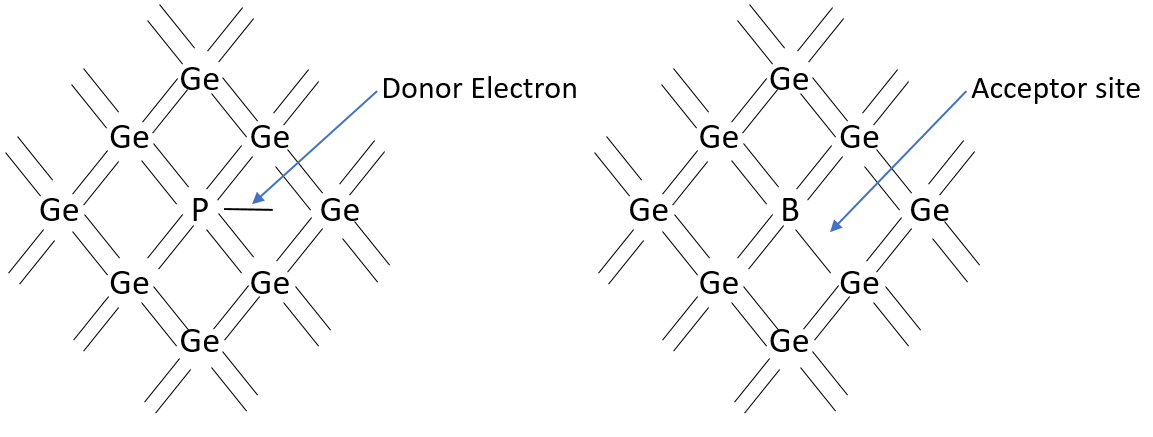
\includegraphics[width=\textwidth]{type}
\caption{Left: example of donor impurity configuration. Right: Example of acceptor impurity configuration}
\label{fig:type}
\end{figure}
An electron can fill an acceptor site where it will be left with a looser bond than the bulk of the crystal.
Whatever carrier is dominant determines the type of material.
Materials where electrons are the majority carrier, such as those doped with phosphorous, are called n-type semiconductors.
When the holes are the dominant information carrier, such as germanium doped with boron, the material is called p-type.

The energy required to create one electron-hole pair is called the ionization energy $\epsilon$.
When a charged particle travels through a detector it creates an amount of electron-hole pairs along its path proportional to the the incident particle energy.
There are always an equal numbers of electrons and holes created during an interaction event which lasts a few picoseconds.
Both carriers need to be fully collected in order to get an accurate energy measurement.

For the semiconductor to be a detector, there needs to be a way of collecting the charge generated by an event.
A typical event that deposits 1 MeV of energy in germanium will generate around $3\times 10^{5}$ electron hole pairs.
If all were drifted with an electric field and collected, it would only generate a current pulse of around $10^{-6}$A.
There needs to be a sufficiently low and stable current through the detector, such that when electron hole pairs are created, the added current pulse can be measured.
Thus it is necessary to have some sort of carrier blocking electrodes.
This will limit the amount of injected charge and current flowing through the bulk of the detector and bring the leakage current to sufficiently low levels.
Leakage current of the system needs to be on the order of $10^{-9}$A in order to be sufficiently low to not interfere with the radiation induced pulse.

In order to have an electric field capable of drifting the electrons and holes at their maximum velocity, the detectors are usually biased to several thousand volts.
This applied voltage can be either negative or positive depending on the detector material type and desired setup.
Once voltage is applied, the electrons and holes will start to drift relative to the field.
Eventually it will get to the point that all of the electrons and holes are split up resulting in one half filled with electrons and the other half with holes.
At this point, the electrons and holes become relatively fixed and there is no further flow of charge in the detector.
Under these circumstances the detector is considered to be fully depleted.

Typical semiconductor diode detectors are able to precisely measure radiation of alpha and beta particles, but have too small of a depletion region to measure the far more penetrating gamma rays.
However, the advent of HPGe detectors allowed for detectors with large volumes to be fully depleted.
Germanium (Ge) is a chemical element and has an atomic number of 32.
It is lustrous and grey in appearance.
It is hard as well as extremely brittle.
Ge is in the carbon group and is classified as a metalloid.
Germanium is most commonly used as a semiconductor in transistors and other electronic devices, notable high-purity Germanium detectors.
Due to its particularly narrow band gap, it has become widely used for radiation detection. 

The working principle of a germanium detector starts with some form of radiation interacting with the germanium and depositing some or all of its energy.
The incoming particle will interact with germanium atoms and cause a certain amount valence electrons, proportional to the energy deposited, to be kicked up to the conduction band.
Due to germanium detectors being operated under high voltage, large electric fields cause the drift of these electron hole pairs to the detector contacts where they can be collected.
This collection of electrons results in an electronic pulse that is amplified, shaped, and finally read out by a computer in the form of an energy spectrum.
\begin{figure}[htpb]
\centering
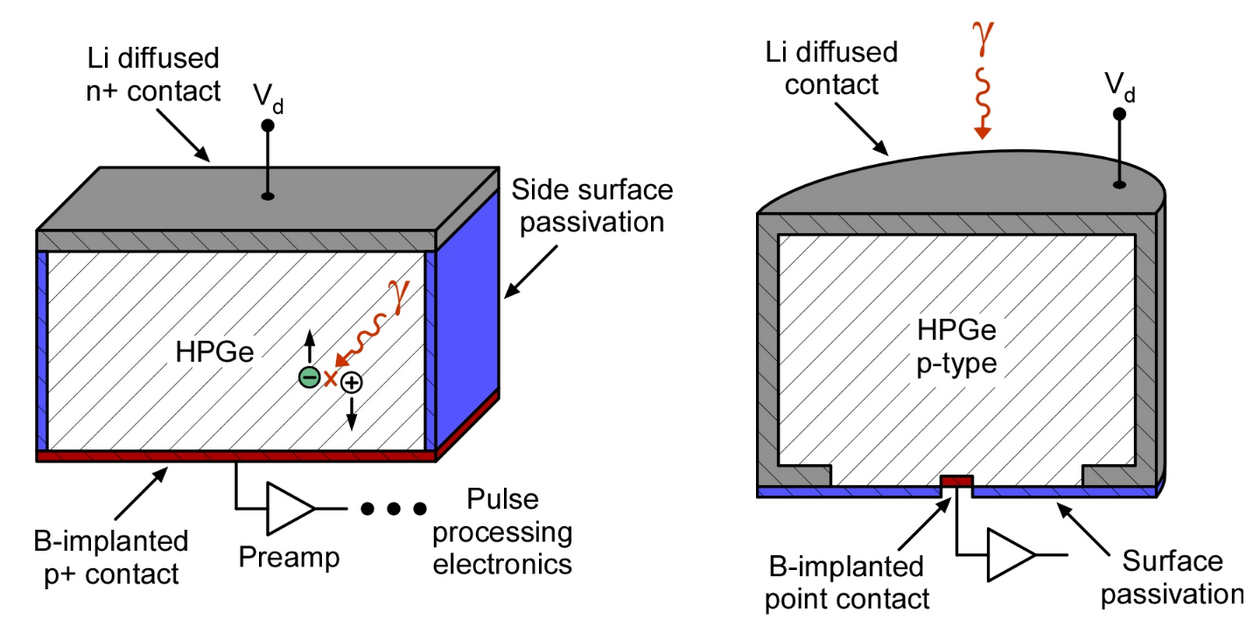
\includegraphics[width=\textwidth]{standard-ge}
\caption{Left: Planar HPGe detector with Li and B contacts. Right: Co-axial detector with Li and B contacts. Photo credit: Mark Amman}
\label{fig:standard-ge}
\end{figure}
Figure \ref{fig:standard-ge} shows a planar HPGe detector which is one of the simplest designs.
In order for the detector to work properly, it must be operated at a high voltage and it must also behave as a capacitor.
Behaving like a capacitor implies that there will be as little leakage current as possible, in other words that there will be no flow of current across the detector.
However, when an interaction happens, the electron hole pairs must be drifted and collected at the contacts.
This means that charge must be able to flow out of the detector but not back in.

It is the role of the detector contacts to provide this blocking of charge injection while facilitating readout of energy from an event.
The most common types of semiconductor contacts are impurity based or amorphous crystal.
For decades, the standard technology was to use a positive n+ lithium contact on one side and a negative p+ boron contact on the other.
The n-type lithium would block hole injection while the p-type boron would block electron injection on the other side due to the coulomb force.
The side surfaces must also be passivated in order to protect the inner material from becoming oxidized and created leakage current problems over time.

\begin{figure}[htpb]
\centering
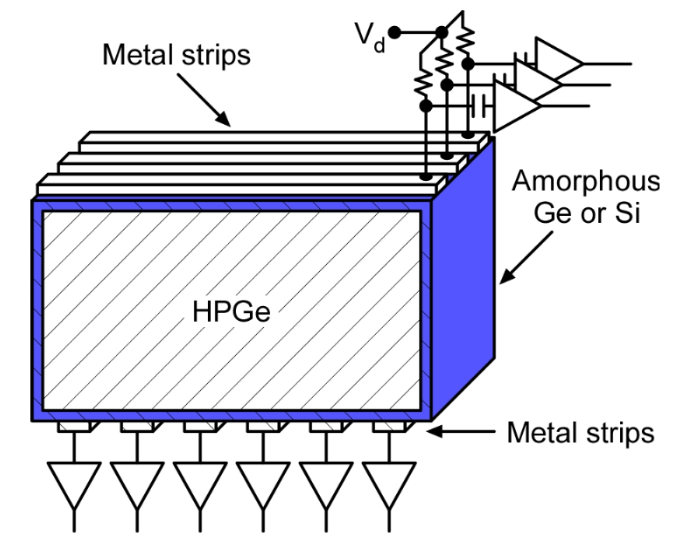
\includegraphics[width=0.6\textwidth]{age-strip}
\caption{HPGe strip detector with amorphous germanium contacts. Photo credit: Mark Amman}
\label{fig:age-strip}
\end{figure}
The problem with lithium diffusion and boron implantation comes when trying implement new designs such as segmented strip detectors.
The lithium diffuses a significant amount into the germanium while boron diffuses less but both leave a dead layer of the detector.
Thus a different type of contact is desired.
It should have a thin dead layer, not diffuse into the crystal, be mechanical robust, and have stable characteristics over time.
One contact method that fits this is an amorphous semiconductor contact such as amorphous germanium.

Amorphous germanium is special because it is bi-polar blocking meaning that it blocks the injection of both holes and electrons due to its effect on the barrier height of the bandgap.
Amorphous germanium can also be used to form the passivation layer on non contact surfaces.
On contact surfaces it provides charge injection barriers, blocking injection of charges from outside the detector, and on the sides it creates a passivation layer. 
Metal such as aluminum can then be deposited on top of the amorphous germanium to provide good electrical contact.



%%%%%%%%%%%%%%%%
% Chapter 4
%%%%%%%%%%%%%%%%

%" vim: fdm=marker:fen:fdl=0
% Manufacturing of Planar Detectors Chapter intro%{{{
\chapter{Manufacturing of Planar Detectors}
The manufacturing process of a planar HPGe detector begins with a slice from a crystal boule that has been tested for quality and is know to be detector grade.
Typical boules slices are solid discs that can range from a few millimeters up to several centimeters in thickness and 5+ centimeters in diameter.
This large size allows for several detector samples to be cut from each slice so careful geometry considerations are important in order to minimize wasted material.
The goal is for the detector sample to look approximately like figure \ref{fig:dummydet} which is an example of a planar detector with so called top hat geometry.
\begin{figure}[htpb]
\centering
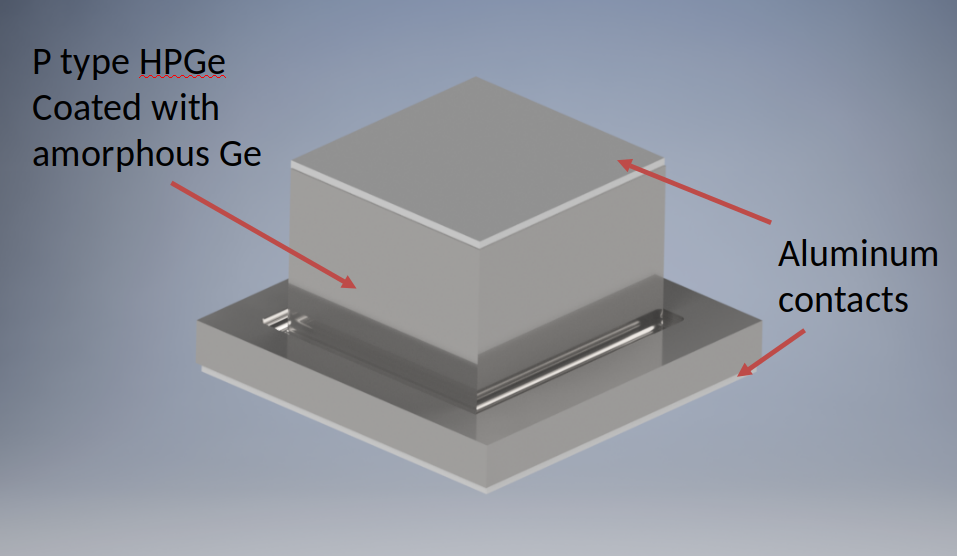
\includegraphics[width=0.5\textwidth]{dummy-det}
\caption{Example detector geometry with four wings}
\label{fig:dummydet}
\end{figure}
The brims of the hat are called wings and serve as a dead area of the detector for handling during the manufacturing process.
The detector is not required to be perfectly square to work so length and width can vary within a few centimeters.
What is of importance are the overall thickness and that the top and bottom faces are parallel.
Due to the relatively long mean free path of gamma rays in germanium, a detector should aim to be at least one centimeter thick.

Once considerations for geometry have been made, the detector manufacturing process begins.
To start, the germanium boule slice is cut into several rectangular cubes.
Then, work proceeds using one of the cubes, saving the rest for the next time.%}}}
% Section: Mechanical Processing%{{{
\section{Mechanical Processing}
The diamond saw under discussion is the SYJ-400 Precision CNC Dicing/Cutting Saw from Shenyang Kejing Auto-Instrument Co.
The structure of this diamond saw is shown below in Figure \ref{fig:diamondsaw}.
It is operated using a CNC controller with setting for the cutting speed, length, time, depth, lifting height, rest time, and movement speed.
All of these parameters are edited using the attached CNC controller. 
There are four separate screens with adjustable parameters that are shown with translations in Figure \ref{fig:control-screen}. 
Each of these parameters are in millimeters or millimeters per minute depending on the operation.
\begin{figure}[htpb]
\centering
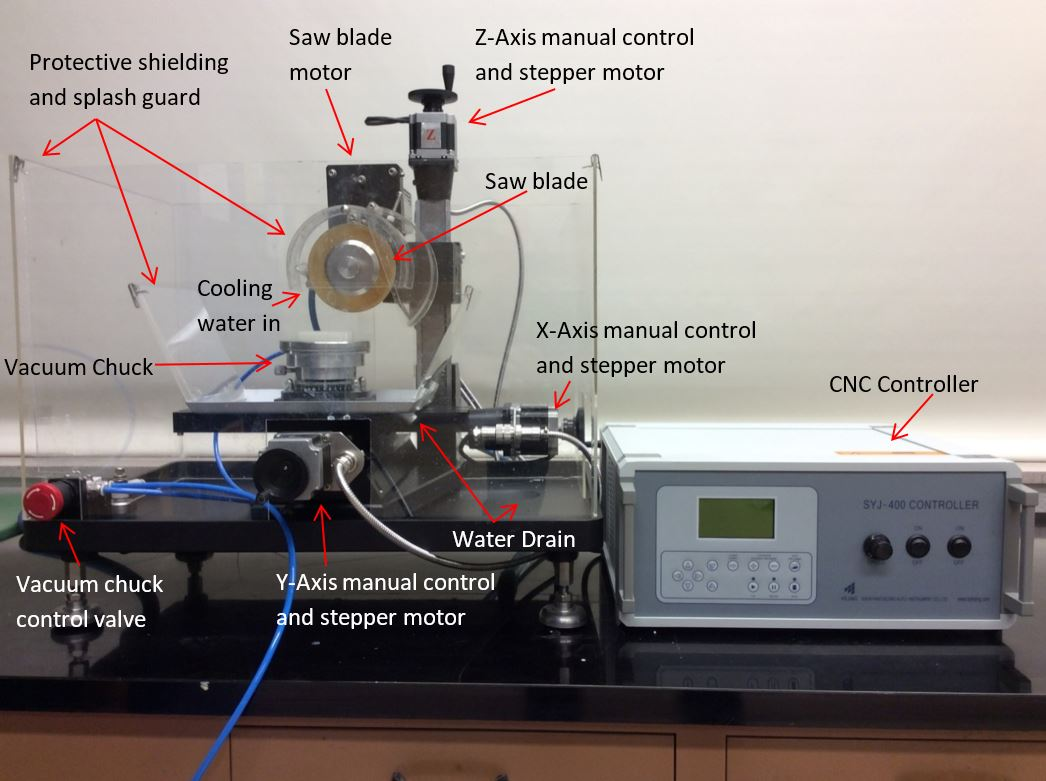
\includegraphics[width=0.8\textwidth]{diamond-saw}
\caption{The diamond saw used to cut boules into detector samples.}
\label{fig:diamondsaw}
\end{figure}

Before turning on the power to the diamond saw, it is important to take care of all of the necessary adjustments such as changing blades and placing the sample onto the vacuum chuck.
It is important to do this before supplying power in order to prevent the saw from somehow starting itself.
To switch blades, first remove the finger screw, labeled 1, on the outside of the splash guard covering the blade. Then remove the finger screw, labeled 2, that holds the blade clamps.
Remove the outer blade clamp and the blade can be switched out.
Depending on the blade size, it may be necessary to change to a larger splash guard.
To do this, first remove finger screw 1 on the outside of the splash guard, then remove the two hex screws, labeled H, on the back plate.
It might be necessary to remove the blade to access these screws.
You can then install the new splash guard and blade working in the opposite order to put everything back together.
\begin{figure}[htpb]
\centering
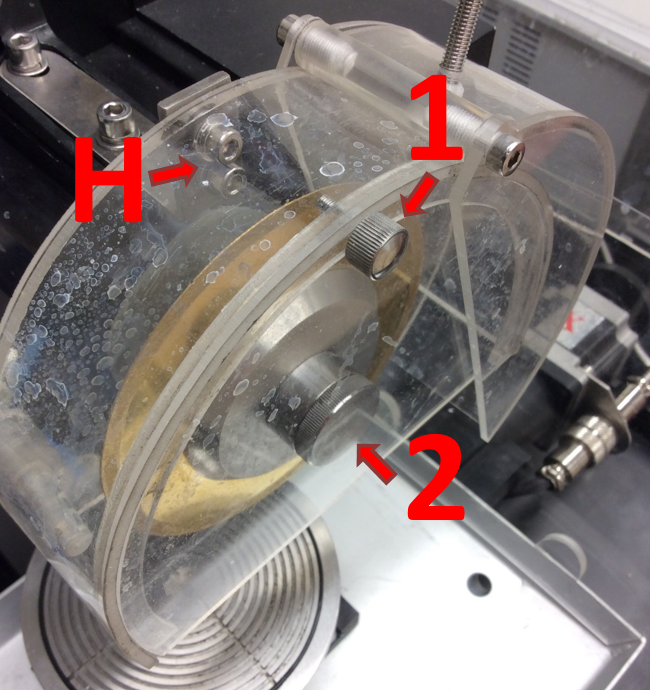
\includegraphics[width=0.5\textwidth]{blade-case.PNG}
\caption{This is the blade and shielding on the diamond saw.}
\label{fig:blade-case}
\end{figure}

There are currently three different blades available for cutting.
They are all four inches in diameter and include: an electroplated diamond blade, full sintered diamond blade, and a 2mm grinding wheel.
The electroplated blade is thin and useful for the initial cuts of the boule.
The grinding wheel is used to make grooves and grind down the detector wings.
\begin{figure}[htpb]
\centering
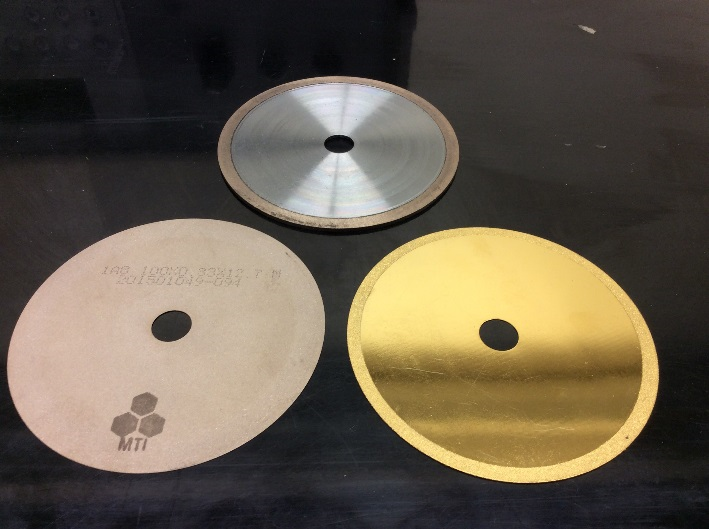
\includegraphics[width=0.5\textwidth]{blades}
\caption{Three different blade types for cutting germanium.}
\label{fig:blades}
\end{figure}

The next step is to mount your sample onto the vacuum chuck.
It is essential to do this before powering on the diamond saw to avoid accidents.
Place the steel sample holder onto the vacuum chuck and adjust it so it is properly aligned.
The vacuum can then be turned on to suction the chuck and keep the sample from moving during cutting.
To start the diamond saw, the power strip must be plugged in and turned on.
The strip will provide power to the vacuum pump and the up/down voltage converter.
The next step is to power on the up/down converter that is located under the table that supports the diamond saw.
The converter will provide a stepped up voltage to the CNC controller (which powers the saw) and the water pump.
The saw controller requires 220 volts which is why it cannot be plugged into a standard outlet.

The first cuts of the boule should be made with the thin diamond blade and go all the way through the germanium into the graphite plate.
The initial cuts are to cut the rough detector shape out of the crystal slice.
An example of a cut boule can be seen in Figure ~\ref{fig:cutboule} where four detector samples are cut from a single crystal.
\begin{figure}[htpb]
\centering
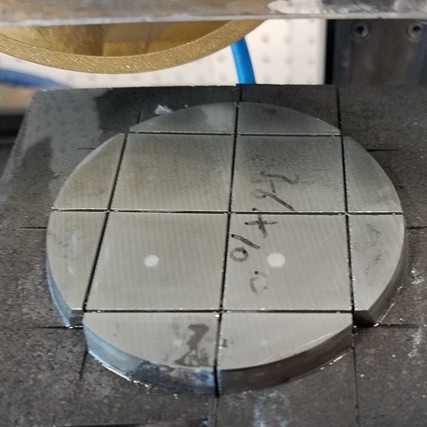
\includegraphics[width=0.5\textwidth]{cut-boule}
\caption{This is the crystal boule after the initial detector sample blanks have been cut.}
\label{fig:cutboule}
\end{figure}
The saw must be start and stopped using the provided controller.
All of the settings and translations can be seen in the appendix in Figure ~\ref{fig:control-screen}.
One property of germanium is that it is an extremely brittle metal.
This can cause problems when cutting because the material will chip under normal cutting speeds.
Due to this problem, the diamond saw must travel less that a millimeter per minute and grind the germanium instead of cutting it.

After the detector blanks have been cut from the boule, the stainless steel and graphite plate are reheated to melt the wax and remove all the extra pieces.
A single detector sample is then left and centered on the graphite for further cutting.
The next step is to replace the thin blade with the grinding wheel so that the groove cuts can be made.
A detector can have either two or four wings depending on the final goal.
The groove are ground out approximately two millimeters from the edge of the sample, then the sample is moved and the remaining bits are ground down to leave the wing shape.
An example of a detector with four wings is shown in Figure ~\ref{fig:cut-sample}.
\begin{figure}[htpb]
\centering
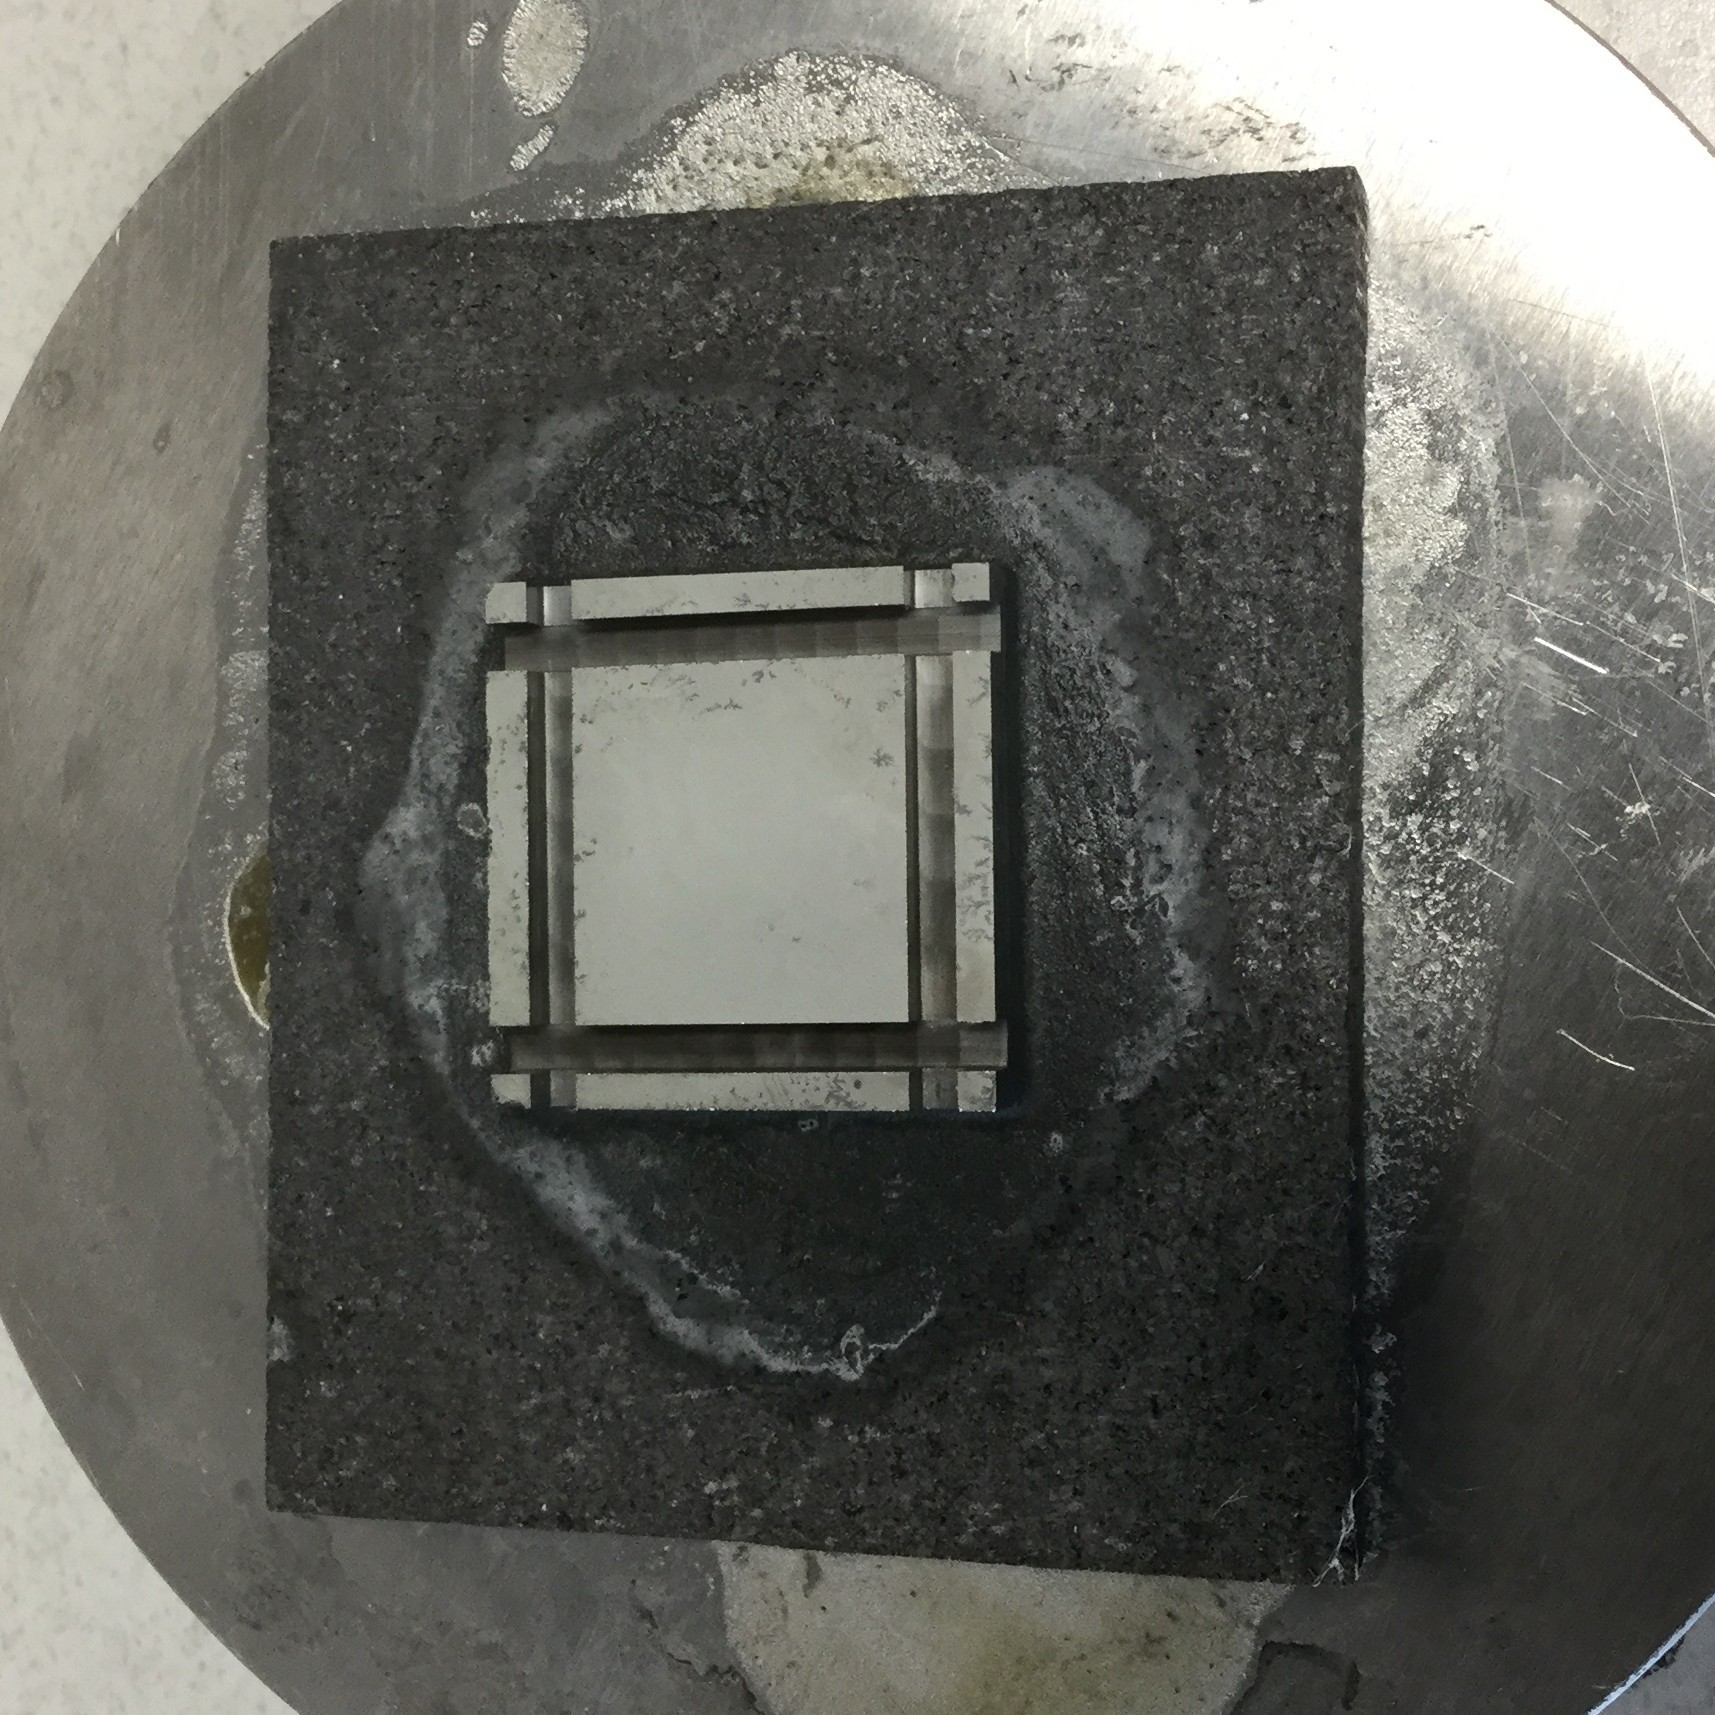
\includegraphics[width=0.5\textwidth]{cut-sample}
\caption{A germanium sample mounted on graphite which is then mounted on a stainless steel chuck.}
\label{fig:cut-sample}
\end{figure}

After the detector has finished up in the diamond saw, it is left with a very rough surface that might have some minor chipping along the edge.
Any cracks or large chips can lead to detector failure down the line so they must be removed before continuing.
The first and most effective way to remove material is through lapping.
For lapping, an abrasive is mixed with water on a glass plate or polishing pad to create a slurry.
Figure \ref{fig:lapping} shows the glass plate with polishing pad on top along with a detector sitting in the slurry.
The detector is then ran across the slurry which slow grinds down the surface.
The speed of material removal is based on the type and particle size of the abrasive.
Two types of abrasives are used for lapping at USD, one is silicon carbide (SiC) and the other is aluminum oxide (Al$_2$O$_3$).
To remove lots of material, the larger grit SiC is used.
The brand ID is Lapmaster 2600 and it has an average particle size of 17.5 micron.
For finer polishing the aluminum oxide with average particle size of 9.5 micron is used.
There 9.5 micron is called Lapmaster 1900.
The Al$_2$O$_3$ is available in several particle sizes where the most used at USD are the 9.5 micron and 1 micron versions.
\begin{figure}[htpb]
\centering
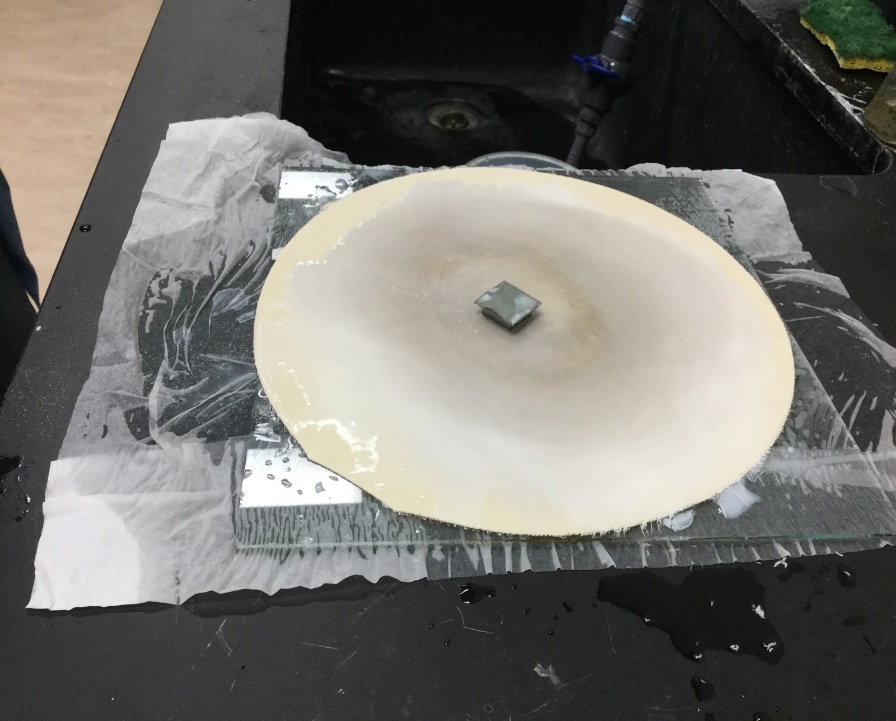
\includegraphics[width=0.5\textwidth]{lapping}
\caption{An example of lapping the detector sample}
\label{fig:lapping}
\end{figure}
Generaly the 9.5 micron Al$_2$O$_3$ is enough to remove major defects from the diamond saw and perpare for chemical polishing.
The standard procedure is to spoon out a few grams of the abrasive onto the glass slide.
Then enough DI water to create a slurry is mixed into the powder.
The detector is then slid around on the slurry which slowly polishes the surface.
Ocassionaly further polishing is required to reduce the amount of time required for chemical processing.
In order to achieve a mirror like finish prior to acid etching, a polishing pad can be used.
When using the polishing pad, shown in Figure \ref{fig:lapping}, it is important to use an abrasive of 3 microns or less to achieve a nice finish.
%}}}
% Section: Chemical Processing%{{{
\section{Chemical Processing}

The cutting and lapping leaves the surface of the detector with micro scratches and defects, sometimes invisible to the naked eye, that could lead to failure down the process line if not treated properly.
Since the next step of detector fabrication involves depositing thin layers of metal that need to stick together, it is important that the surface is as smooth and clean as possible.
Acid etching is a useful tool to remove the outer layer of germanium and leave behind a smooth and defect free surface as long as the right chemical mixture is used.  

Several chemical treatments are commonly used in the semiconductor industry to deal with such cleaning and polishing.
For cleaning there are solvents such as acetone, methanol, and Trichloroethylene that are used to remove the wax and debree after cutting.
The detector manufacturing lab is equipped with a metal hood for such operations involving these solvents that is shown in Figure ~\ref{fig:metalhood}
\begin{figure}[htpb]
\centering
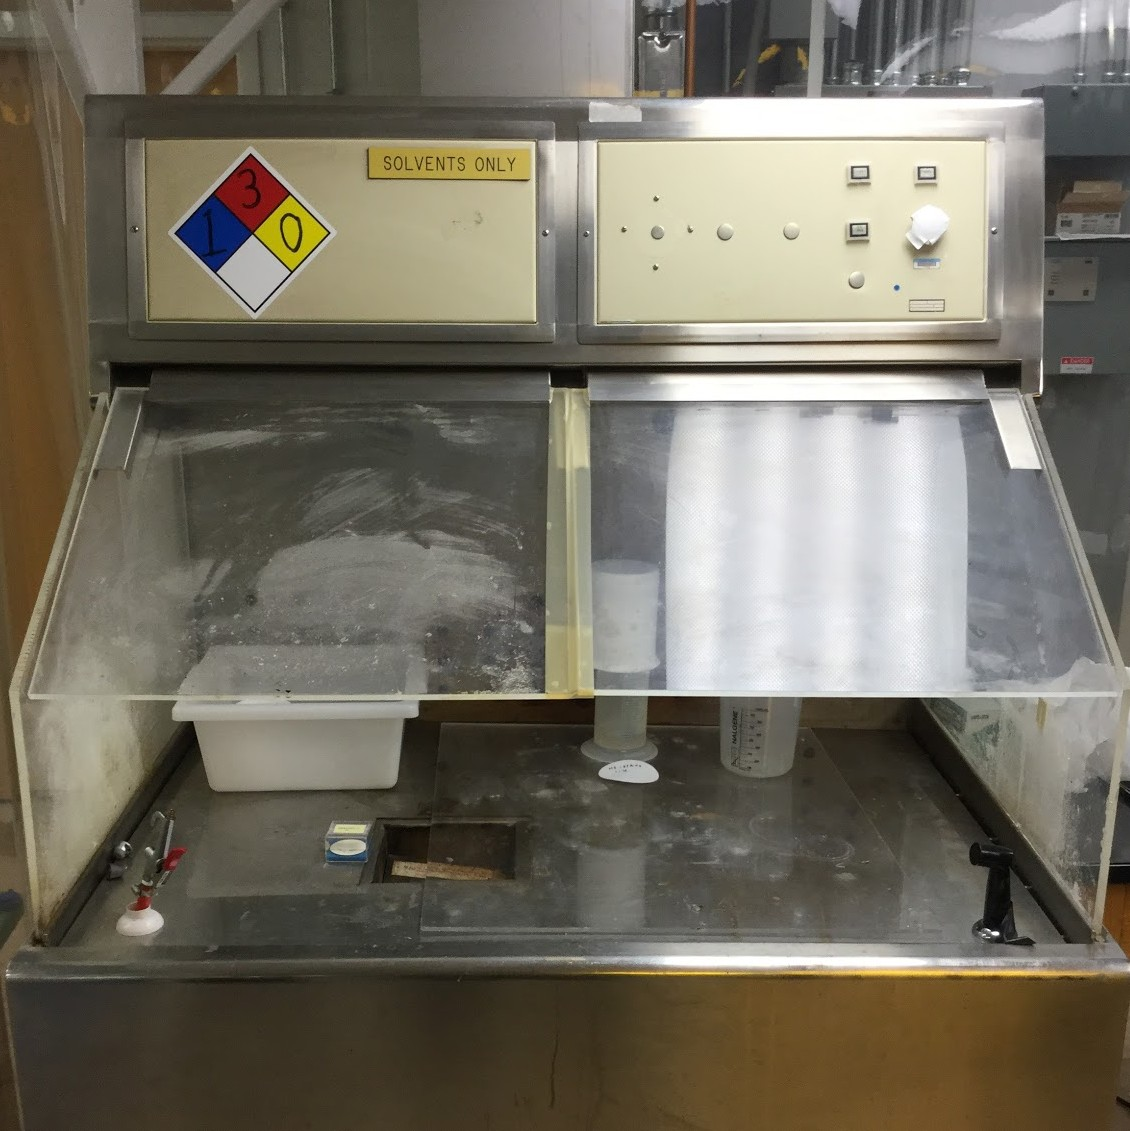
\includegraphics[width=0.5\textwidth]{metal-hood}
\caption{Metal hood for use with solvents}
\label{fig:metalhood}
\end{figure}

For polishing it is standard to use an acid etch, usually a mixture of Nitric (HNO$_3$) and hydrofluoric (HF) acids.
The ratio of the two acides will determine how agressive the etch is.
For detector fabrication a 4:1 HNO$_3$:HF ratio is used.
Figure \ref{fig:plastichood} shows the plastic hood that is used for acid etching.
\begin{figure}[htpb]
\centering
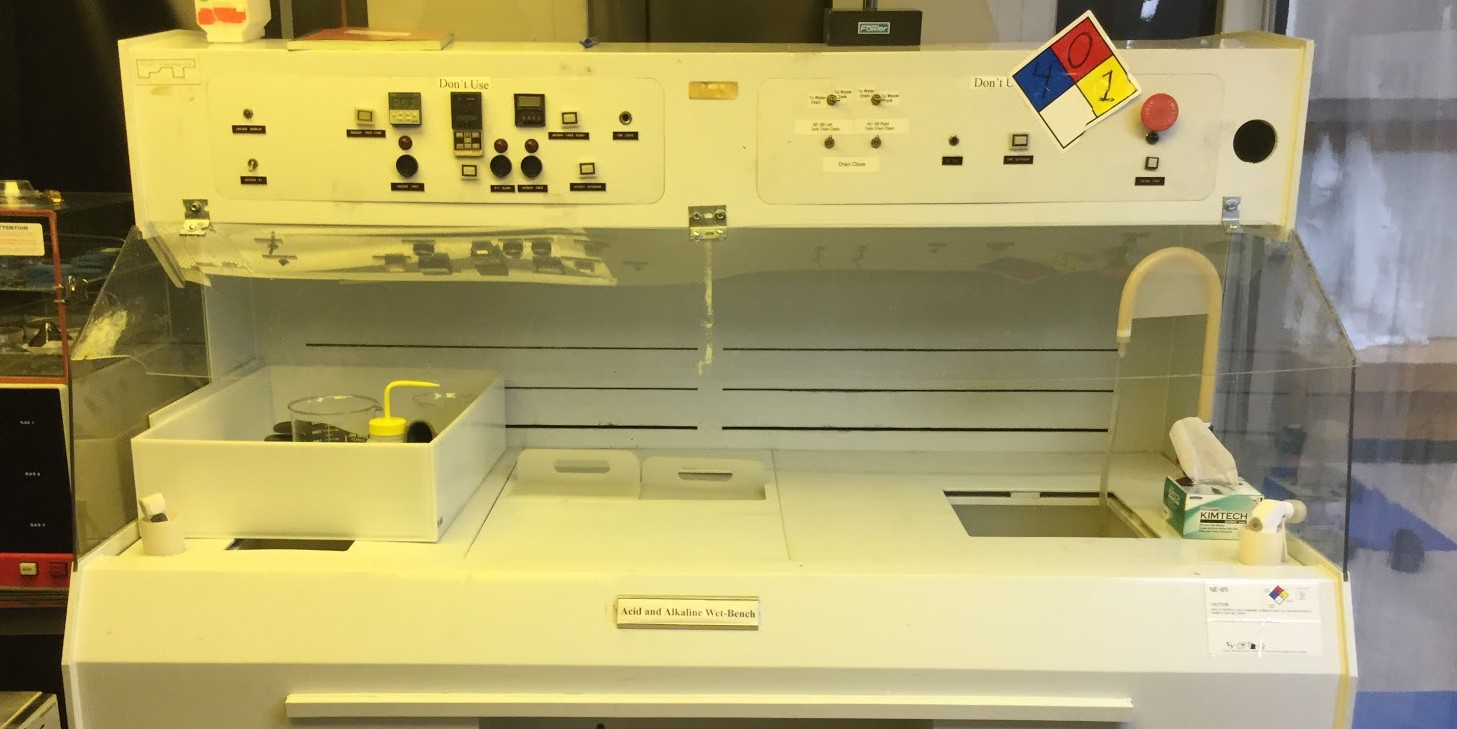
\includegraphics[width=0.7\textwidth]{plastic-hood}
\caption{Plastic hood for use with acids.}
\label{fig:plastichood}
\end{figure}
To prepare for sputtering and aluminum deposition, two etches are required.
Both etches are in the 4:1 solution, however, the time varies.
The first etch is around three minutes long and takes place after lapping.
This longer etch is meant to fully polish the crystal and rid it of scratches and defects.
The second etch is only 30 seconds and is to clean the surface of the crystal immediately before it is loaded into the sputtering machine.

The procedure for acid etching starts with taking proper precautions to ensure safety and prevent accidents.
Heavy duty gloves are worn overtop several layers of lab gloves, along with safety goggles, lab coat, and respirator if necessary.
Then the acid mixture can be made.
Figure \ref{fig:acidbeakers} shows the acid bottles along with several beakers and a graduated cylinder.
The graduated cylinder is used to measure out the proper ratio of acids, usually 160 ml of nitric acid is poured in first followed by 40 ml of hydrofluoric.
This is enough solution for at least two etches.
Approximately 100 ml of solution is then poured into an empty PTFE beaker.
It is also necessary to have at least three beakers filled with DI water, two for quenching after the etch and one two quench any paper waste.
\begin{figure}[htpb]
\centering
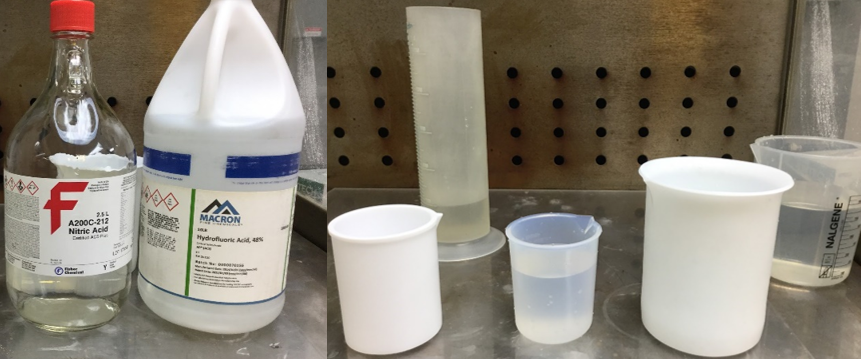
\includegraphics[width=\textwidth]{acidbeakers}
\caption{Left: Nitric and Hydrofluoric acid bottles. Right: Graduated cylinder PTFE and plastic beakers}
\label{fig:acidbeakers}
\end{figure}
After the setup is complete, etching can proceed.
For the longer three minute polish, the clean detector sample is placed in the acid using longacid resistant tweezers.
The detector must then be continuously agitated and flipped halfway through to ensure a uniform etch.
After the three minutes have elapsed the detector is removed and immediately dipped into the first DI water beaker for a few seconds to stop the etch.
Then it is dipped into the second DI water beaker to remove any remaining acid.
After the DI water quench, the detector is quickly dried with dry nitrogen to remove all moisture from the surface.
The surface of the detector sample should now have a mirror finish, although some minor cloudiness sometimes arises and is acceptable.
If scratches remain, the detector can be etched further, usually for a minute or less.
\begin{figure}[htpb]
\centering
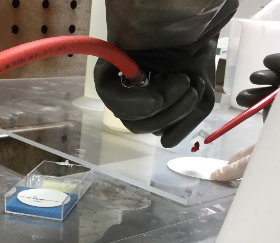
\includegraphics[width=0.5\textwidth]{drynitrogen}
\caption{A detector sample being held and dried with nitrogen.}
\label{fig:drynitrogen}
\end{figure}

At this point the detector sample is ready for the final 30 second etch and loading into the sputtering machine.
The same etch mixture is used as in the long etch, only this time the sample is held continuosly by the tweezers and is swished around in the acid.
Being held continuously prevents the surface from contacting anything other than acid and keeps it free from the possibility that more scratches are introduced.
The steps of quenching in DI water and drying with nitrogen are the same with importance being placed on the sample being held and never allowed to touch any surfaces.
After the detector sample is dried, it can be placed onto the sputtering jig and loaded into the sputtering machine.
%}}}
% Section : Amorphous Ge Deposition%{{{
\section{Amorphous Ge Deposition}

Need information on the working principles of sputtering machine
also need more on the range measurement, marks papers citing specific values for settings 
\subsection{Principles of Sputtering}

\subsection{Operating Procedure}
The sputtering machine at USD is a Perkin-Elmer 4400 Sputtering System.

The operating procedure for the sputtering machine is complex and care is required to make sure the system maintains working order.
It is a complex system with multiple valves, controls, power supplies, vacuum systems, and pressure monitors that all work in conjunction to deposit a thin layer of amorphous germanium on the detector sample.
One key component of the system is a cryopump that uses pressurized helium gas to quickly vacuum the system to the proper pressure.
The cryopump system can be seen in Figure ~\ref{fig:sput-flow} as blue boxes with labels connected by green lines.
The green lines exchange the helium between the cold head connected to the vacuum chamber and the compressor located in the pump room.
Before the sputtering procedure can begin, the cryopump must be turned on to allow the cold head to cool from room temperature to approximately 20K.
Prior to cooling down the cryopump, it must be vacuumed to below 100 mtorr using the rough pump describe later.
In order to vacuum the cryopump, open the forline valve shown as E in ~\ref{fig:sput-flow}; close the valve before turning on the cryopump.
The on/off switch for the compressor is located on the panel with the other valve toggles and is labeled as "HY-VAC PUMP"

Once the cryopump is cooled down to the proper temperature, the sputtering procedure can begin.
As seen in Figure ~\ref{fig:sput-flow}, there are multiple valves for opening and closing various gas and vacuum lines.
These valves are all pneumatically opened and closed so they require a constant supply of pressurized air at 60 psi.
This pressurized air is supplied by a large Kaeser SX 5 compressor located in the pump room and shown in Figure ~\ref{fig:comp-air}.
\begin{figure}[htpb]
\centering
\includegraphics[width=\textwidth]{comp-air}
\caption{Kaeser SX 5 compressor}
\label{fig:comp-air}
\end{figure}
The compressor is turned on or off by pressing the green or red button on the control interface shown on the top left side of the figure.
Once turned on, it will automatically increase in pressure until it reaches a set point around 100 psi.
The pressure out is then reduced or increased by adjusting the pressure regulator shown on the bottom left.
It is important to check the pressure often to make sure that it is sufficiently high for if it drops too low, valves will return to the default closed position.

Once the system has been supplied with pressurized air, the valves can be opened or closed and the system is ready to be operated.
The next step is to load the detector sample into the sputtering machine and prepare for deposition.
The sputtering system should always be kept under vacuum so before it can be opened it must be returned to standard atmospheric pressure.
This is done by opening the vent valve and filling the chamber with dry nitrogen.
The toggle switch for the vent valve is located at 'A' in Figure ~\ref{fig:sput-flow}.
The nitrogen in routed in from a tank located in a separate room behind the pump room and is kept at approximately 10 to 15 psi.

After the chamber has returned to atmospheric pressure it can be opened using a hydraulic lift system that is powered through the RF power generator.
The sample can now be carefully placed inside the chamber centering it under the amorphous germanium target as seen in Figure ~\ref{fig:sput-open}.
\begin{figure}[htpb]
\centering
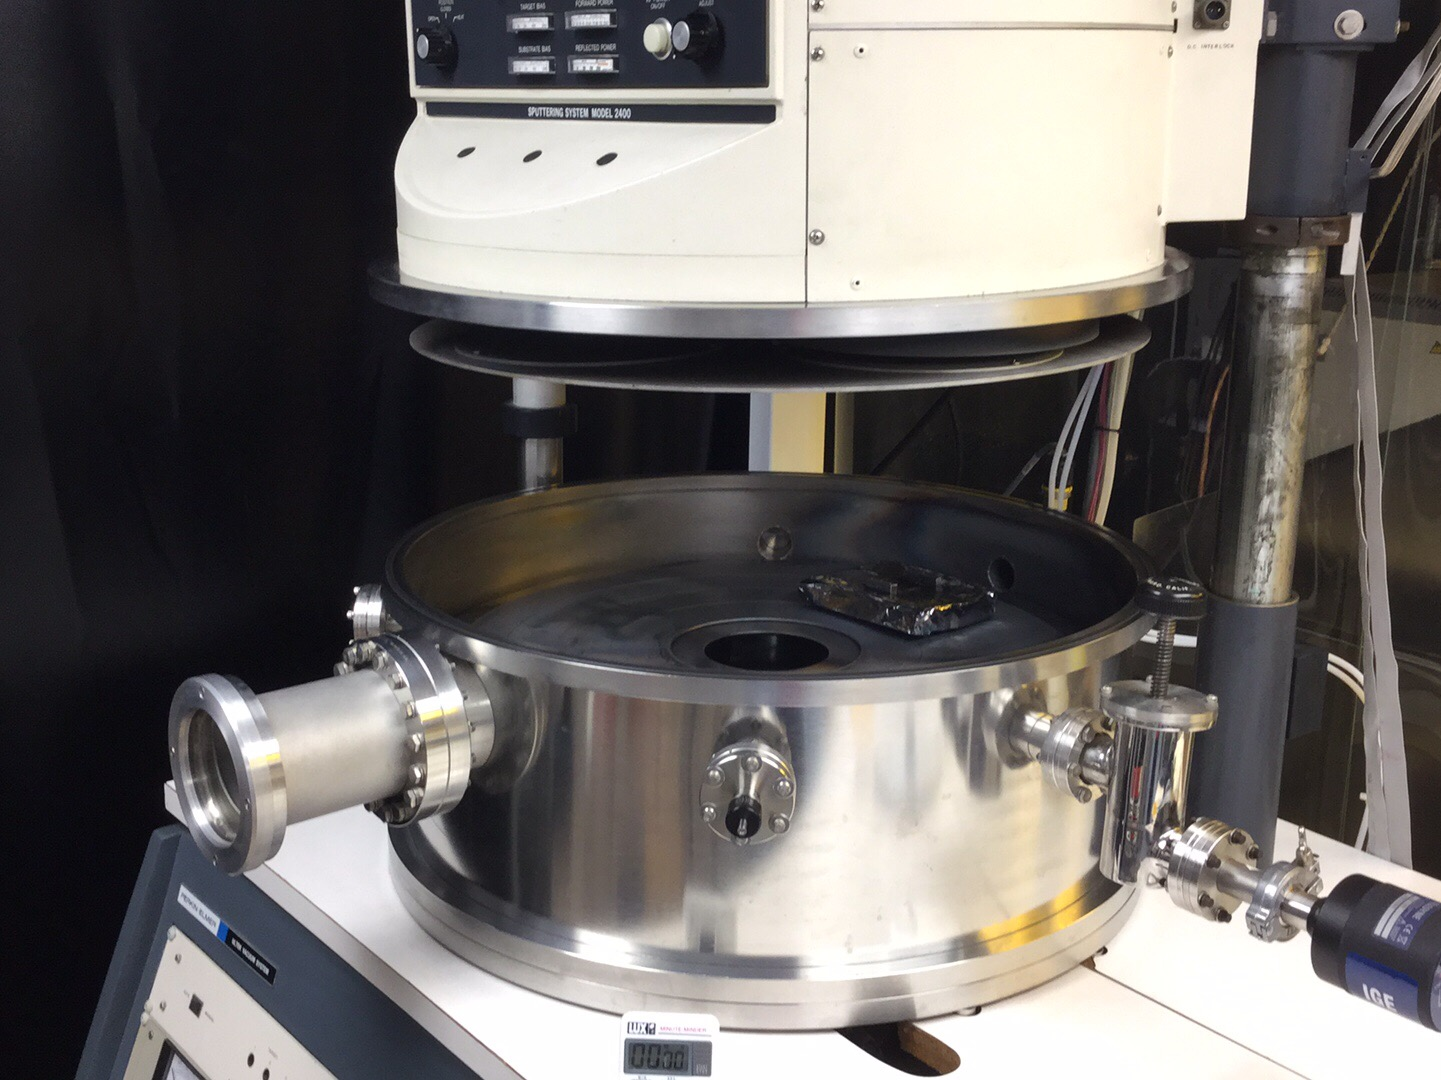
\includegraphics[width=0.6\textwidth]{sput-open}
\caption{Sputtering machine with chamber open}
\label{fig:sput-open}
\end{figure}
A jig is used to hold the detectors by the wings during the sputtering process.
It is designed to be adjustable, allowing for various detector sizes and geometries.
After the detector sample has been chemically etched it can be loaded onto the jig and then into the sputtering machine.

Once the sample is loaded the chamber can be closed and vacuum pumping can begin.
The first stage of pumping is done by a rough pump which takes the chamber from atmospheric pressure down to below 100 millitorr.
The rough pump is turned on or off by switching an electrical breaker located outside of the clean room.
After the pump is on and running normally, the roughing valve can be opened.
Opening the roughing valve allows the rough pump to vacuum the chamber from atmospheric pressure to around 100 mTorr.

Once the chamber has reached some pressure between 50-100 mTorr the roughing valve can be closed and the HY-VAC VALVE, shown as D in Figure \ref{fig:sput-flow}, can be opened.
The cryopump will then be able to vacuum the system to the required $10^{-6}$ Torr for sputtering.
The sputtering machine takes less than five minutes to go from atmosphere to $10^{-3}$ Torr using the rough pump and a further 2-3 hours to reach $10^{-6}$ Torr using the cryopump.

After proper vacuum pressure is achieved the sputtering deposition procedure can start.
The first thing is to start the water chiller and make sure the proper lines are selected.
The chiller is used to provide cooling to the target and stage during deposition as the plasma generates considerable heat.
It is located in the pump room and is show in Figure ~\ref{fig:water-cool}.
The middle picture of the figure shows the side view of the chiller where the separate lines to the sputtering and e-beam machines are visible.
The selection of lines is done by switching two valves on the back of the water chiller.
The handles of the valves indicate the direction of flow and is used to determine which line is selected.
\begin{figure}[htpb]
\centering
\includegraphics[width=\textwidth]{water-cool}
\caption{Water chiller for cooling the sputtering machine and e-beam evaporator}
\label{fig:water-cool}
\end{figure}

Once the water chiller has reached the set point temperature of \SI{10}{\celsius}, the deposition can start.
First the RF power supply should be turned on by flipping the switch at the base of the front.
The throttle valve, shown as C in Figure ~\ref{fig:sput-flow}, can now be turned on to limit the vacuuming of the chamber.
Now the mixed gas can be vented into the chamber using the gas flow adjuster show in the figure.
To the left of the flow controller is the togle switch to open the mixed gas line.
Then, the flow controller is turned on and set to approximately 50 SCCM.
Due to the throlle valve being on, the chamber will begin to increase in pressure based on the flow controller setting.
The key is to adjust the flow rate until a steady 14 mTorr chamber pressure is achieved.

After the chamber has stabalized at 14 mTorr the RF power can be introduced to the gas in order to generate the plasma required for sputtering.
This is done by pressing the power on button at the top of the chamber show in Figure.
The power can then slowly be increased to the marked point.
During this increase in power, the tune and load must be adjusted to keep the reflected power to a minimum and make sure all the power is transfed into the gas.
At a certain point, the plasma will form and the reading for forward and reflected power will jump up.
It is again necessary to quickly readjust the tune and load to get the reflected power back to 0.
After the reflected power is reduced, the power can be further adjusted to the required level, usually around 100 watts.
Once the plasma is generated, the user must wait for at least five minutes with the shutter closed to bombard the target and clean off the outer layer.
After this five minutes the shutter can be opened which will start deposition on the sample.
The machine can then be run for 15 minutes with the shutter open.
After 15 minutes have elapsed, the RF power can be turned off.
The detecor sample should have accumulated a layer of amorphous germanium that is around 300 nm thick.

The machine can then be opened up and the sample flipped over to coat the other side.
This is done by first turning down the flow rate of the mixed gas to zero and closing the valve.
Then the throttle valve can be turned off followed by closing the HY-VAC VALVE.
At this point the chamber should no longer be pumping so the vent valve can be opened and the chamber returned to atmospheric pressure.
The sample can then be flipped and the sputtering process starts again with closing the chamber and rough pumping.
\begin{sidewaysfigure}
\includegraphics[width=\textwidth]{sput-flow}
\caption{This is a diagram of the Sputtering machine vacuum and gas system. Each valve is connected to a pressurized air line.}
\label{fig:sput-flow}
\end{sidewaysfigure}%}}}
% Section: Aluminum deposition%{{{
\section{Aluminum Deposition}
\subsection{Principles of e-beam}
\subsection{Operating Procedure}
Once the detector sample has been completely coated with a layer of amorphous germanium, aluminum can be deposited on the top and bottom surface to create the electrical contacts.
The aluminum serves as the electrical contact and covers the entire surface of the top and bottom which is what defines the detector as planar.

The e-beam has two separate power supplies: one for powering the controls and vacuum system, and another for supplying the high voltage to the electron gun.
To initiate the startup procedure, the control power supply is turned on.
Afterwords the controlls can be activated by switching the selector from 0 to 1 as seen in Figure \ref{fig:vac-control}.
This will supply power to the vacuum system which needs to be activated by following the prompts on the the screen.
Pressing start will initialize the system, activating the rough and turbo pump.
Once the turbo pump has reached 42 krpm it is ready to vacuum.
\begin{figure}[htpb]
\centering
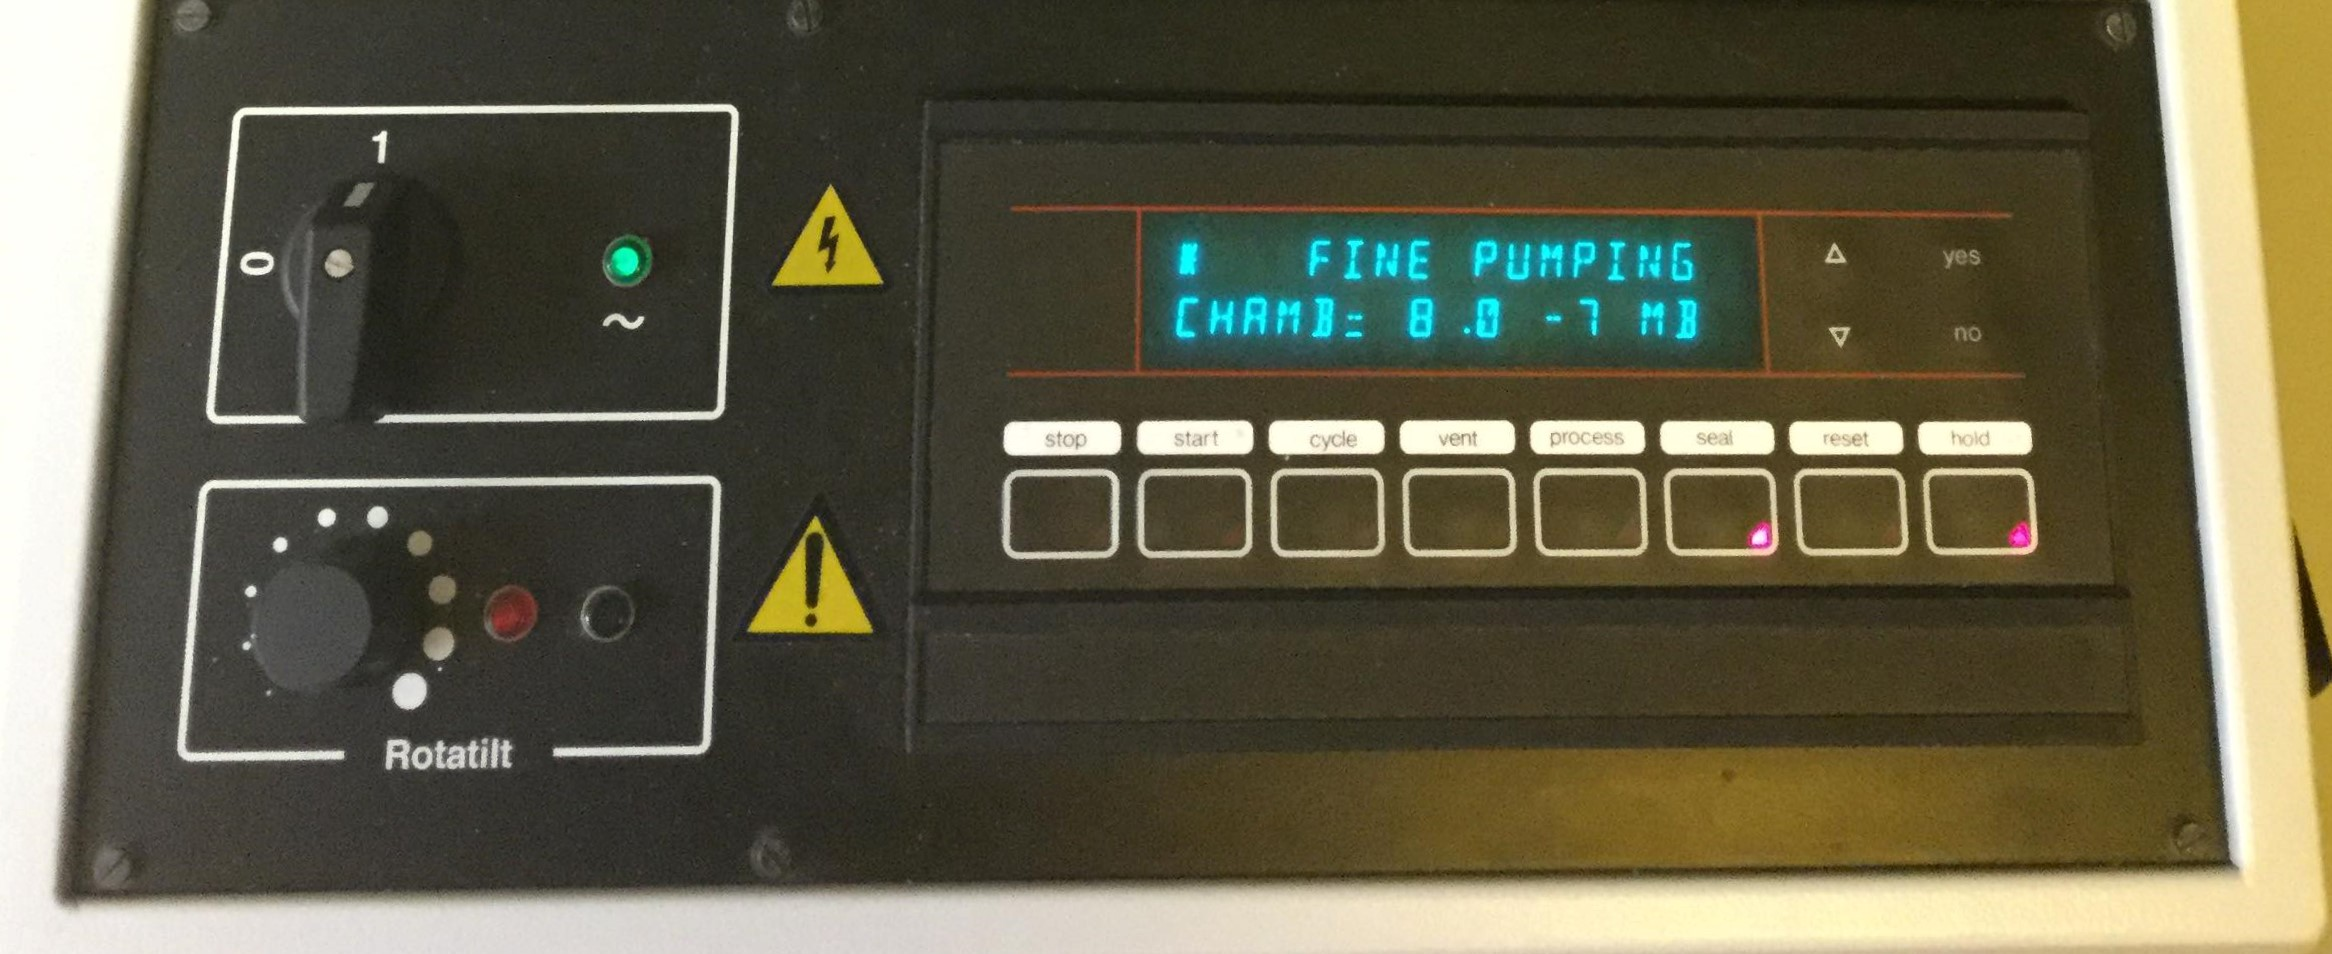
\includegraphics[width=\textwidth]{vac-control}
\caption{E-Beam vacuum controls and power switch}
\label{fig:vac-control}
\end{figure}

The vacuum pumps are located in a cabinet directly under the e-beam chamber as shown in Figure \ref{fig:ebeam-flow}.
The turbo pump has a separate controller that displays the speed which can be seen when the cabinet is opened.
Pressing seal will isolate the turbo pump from the chamber and allow it to be vented so the sample can be placed inside.
Once sealed, the vent button can be pressed which will open the valve allowing nitrogen to fill the chamber.
After the chamber has reached atmospheric pressure the door will be able to open and the sample can be placed loaded onto the holder shown in Figure \ref{fig:ebeam-holder}.
The holder can then be secured inside the chamber using a hex screw and wrench.
\begin{figure}[htpb]
\centering
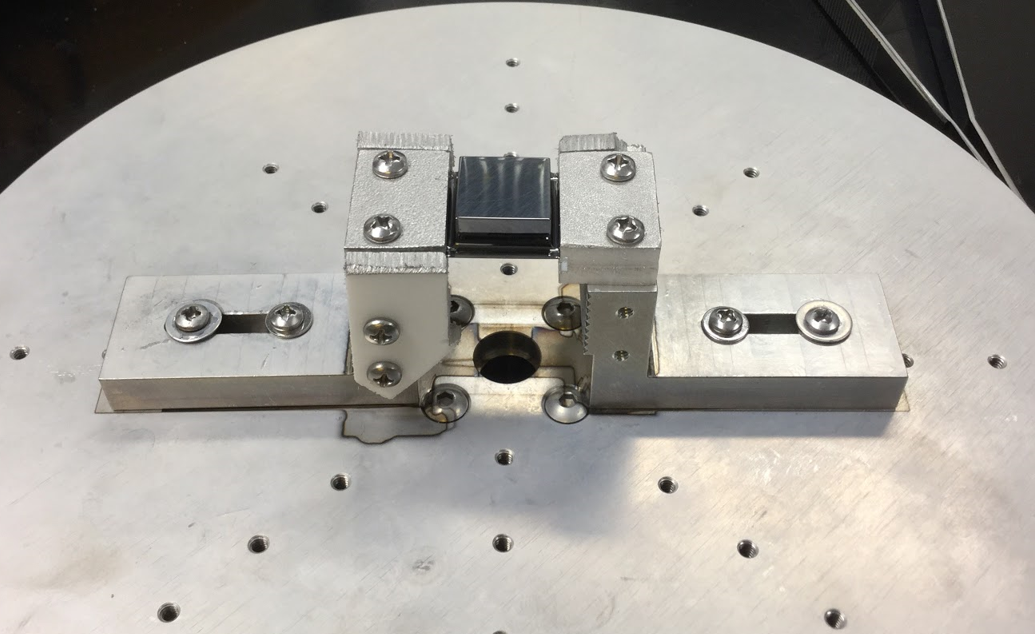
\includegraphics[width=0.6\textwidth]{ebeam-holder}
\caption{Sample holder for the E-Beam}
\label{fig:ebeam-holder}
\end{figure}
Once the sample is loaded, the chamber door can be closed and the the process button pressed.
This will open up the chamber to the vacuum system and start the rough pump.
Once the vacuum has reached sufficient level, the turbo pump will automatically turn on.
The vacuum must reach around $10^{-6}$ torr before the aluminum deposition can start.

Once the proper pressure is reached, the aluminum deposition can begin.
To start, the electron gun power supply is turned on by flipping the switch on the front panel of the high voltage power supply.
Then the on/off switch on the source control, shown in the upper right of Figure \ref{fig:source-control}, can be switched on.
The gun button can then be depressed.
This will provide around 4.9 kV to the electron gun, however, the current remains at 0 so there is no flow of electrons yet.
The current can then be turned up slowly using the dial labeled current.
\begin{figure}[htpb]
\centering
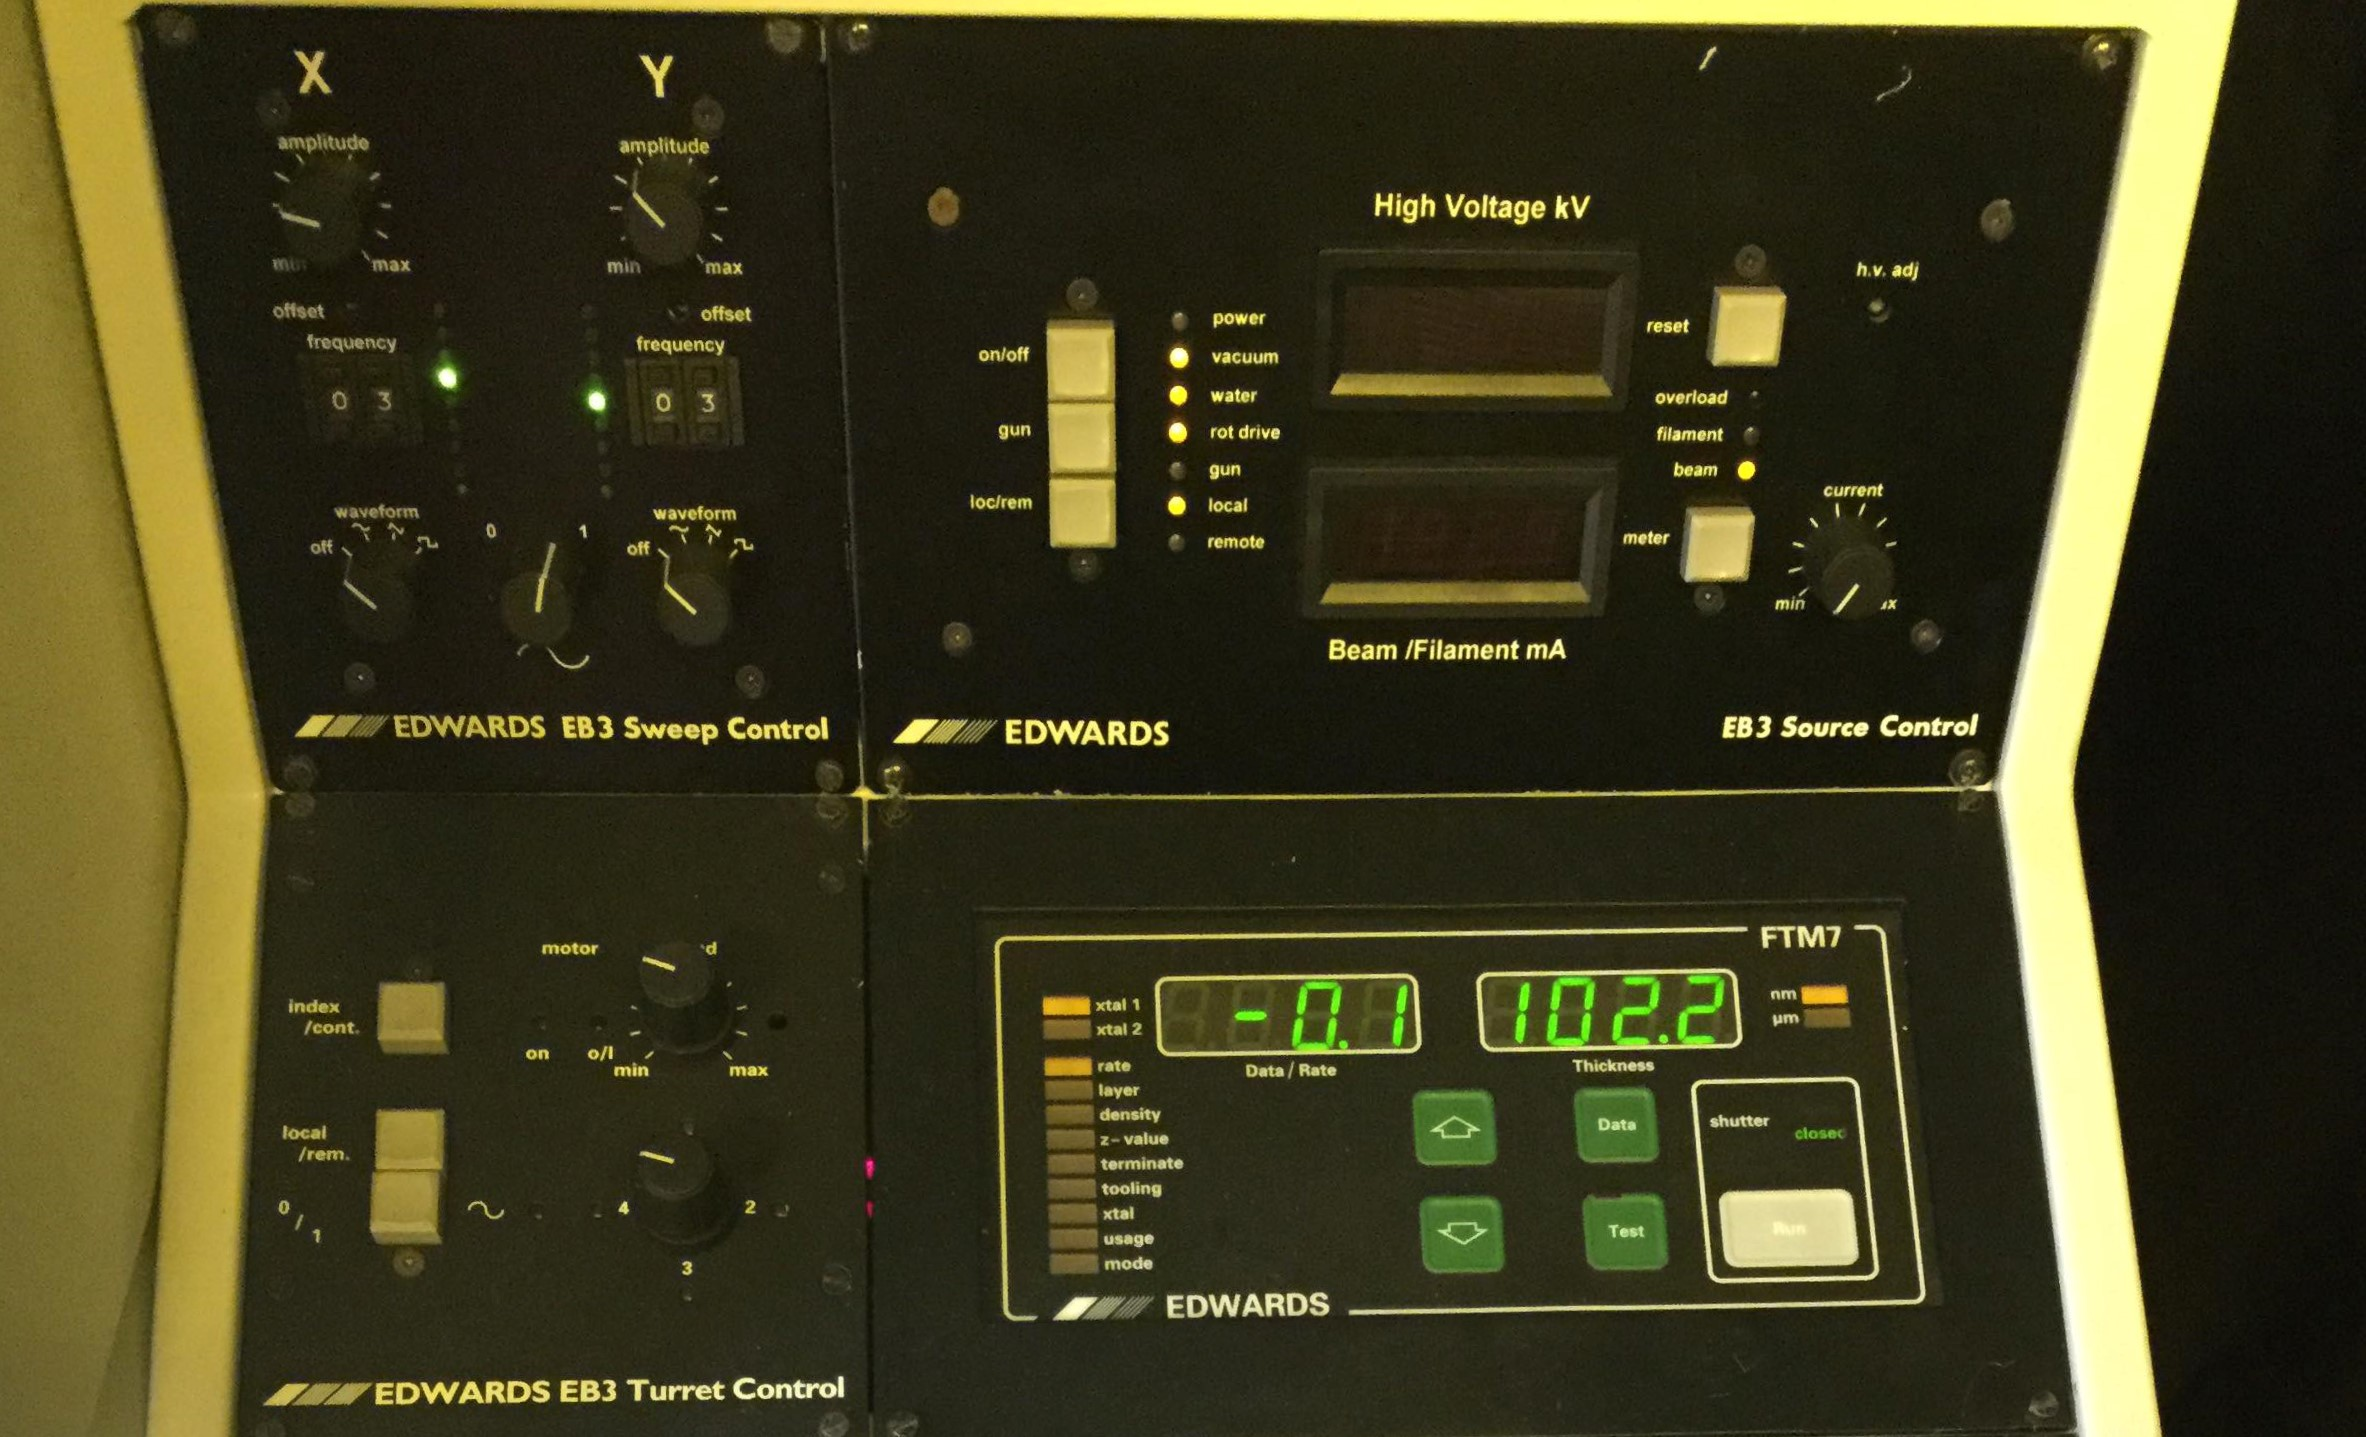
\includegraphics[width=\textwidth]{source-control}
\caption{E-Beam controls for the electron gun, sweep, crystal monitor, and crucible select}
\label{fig:source-control}
\end{figure}

Once the current has reached around 17 mA, the sweep control can be turned on by switching the dial from 0 to 1.
The current can then be continued to increase until the Data/Rate of the crystal monitor is a steady 0.1-0.2 nm/min.
Once the deposition has stabalized, the shutter can be opened by pressing run on the FTM7 controll panel.
This will automatically open the shutter until the predefined thickness, usually around 100nm, is reached.
The shutter will then automatically close and the current can slowly be reduced to zero.

\begin{sidewaysfigure}
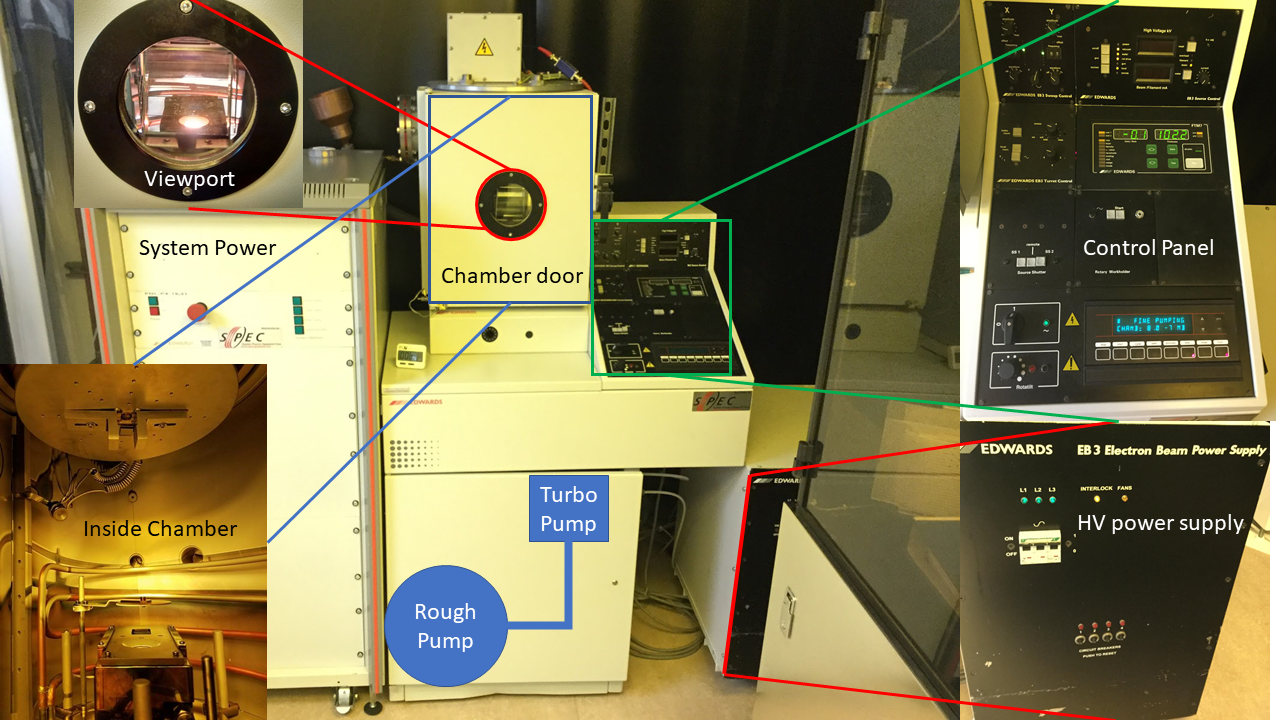
\includegraphics[width=\textwidth]{ebeam-flow}
\caption{This is a diagram of the of the electron beam machine.It is used to deposit aluminum onto the detector sample.}
\label{fig:ebeam-flow}
\end{sidewaysfigure}
%}}}
% Section: Final Steps%{{{

\section{Final Steps}
The nature of e-beam deposition usually leaves the entire chamber coated with aluminum, including the side surface of the detector sample.
While aluminum is great for the contacts, it can cause the detector to breakdown if any is left on the surfaces other than the contacts.
Thus after aluminum deposition, the sides must be etched with acid to remove any aluminum before the detector can be tested.
However, this etch must not attack any of the aluminum left over on the surface.
To prevent this from happening, a mask of tape is placed over the top and bottom surfaces before etching as seen in Figure \ref{fig:taped}.
The tape used is acid resistant and has low adhesian so that the surface will not be damaged and no residue will be left after it is removed.
\begin{figure}[htpb]
\centering
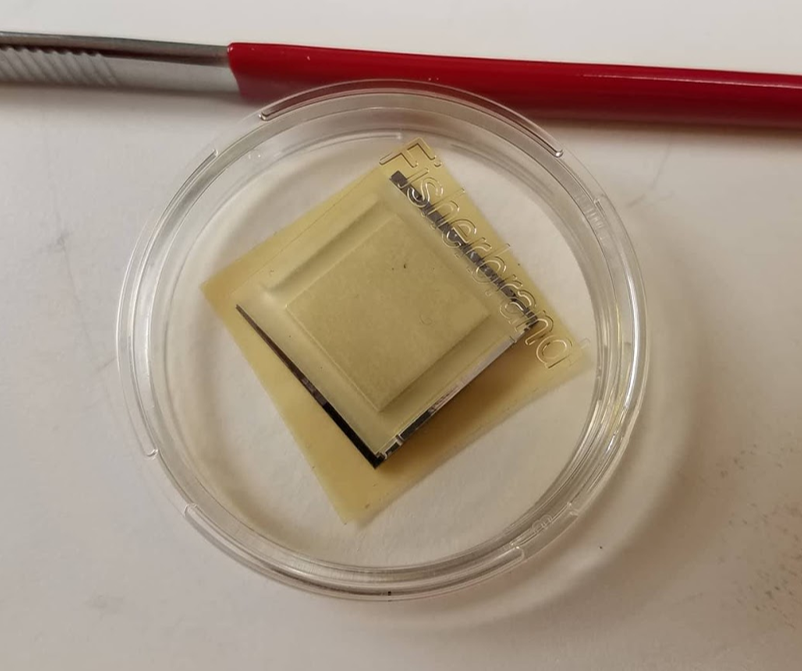
\includegraphics[width=0.5\textwidth]{taped}
\caption{Detector with tape masking before etching.}
\label{fig:taped}
\end{figure}

The taped sample is dipped in 1\% HF for a few minutes until all of the aluminum has been etched away.
The HF does not attack germanium so the amorphous germanium blocking layer beneath will be untouched.
After the aluminum is etched away, the tape is carefully removed using a Q-tip and tweezer being careful to not scratch the surface.
The detector is now complete and can be loaded into the cryostat for testing.

%}}}


%%%%%%%%%%%%%%%%
% Chapter 5
%%%%%%%%%%%%%%%%

" vim: fdm=marker:fen:fdl=0
\chapter{Thin Film Deposition}
% Section : Amorphous Ge Deposition%{{{
\section{Amorphous Ge Deposition}

Need information on the working principles of sputtering machine
also need more on the range measurement, marks papers citing specific values for settings
\subsection{Principles of Sputtering}
Sputter deposition is a method of thin film deposition that works well for certain metals such as amorphous germanium.
Sputtering works by ejecting atoms of a "target" material onto some other substrate.
Figure \ref{fig:sput-theory} shows a graphic of the sputtering process.
The chamber is first vacuumed and then pressurized using a gas, usually argon.
Power is then transferred to the gas which ionizes it and creates a plasma.
The gas ions are then accelerated towards the target due to the electric field inside the chamber.
The ions bombard the target which then ejects neutral atoms which are deposited on the substrate and chamber walls.

\begin{figure}[htpb]
\centering
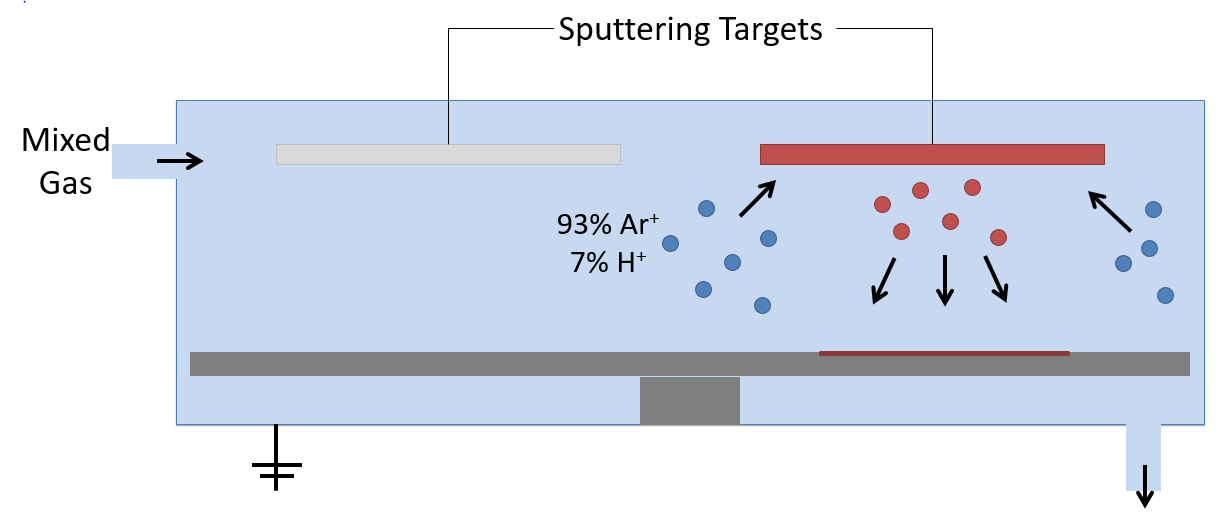
\includegraphics[width=0.8\textwidth]{sput-theory}
\caption{Caricature of the sputtering process}
\label{fig:sput-theory}
\end{figure}

\subsection{Sputtering Calibration}
The amorphous germanium layer must achieve a minimum thickness in order to operate correctly.
Thus it is necessary to evaluate how much AGe is deposited during normal operating procedure with typical settings that would be used during detector fabrication.
The sputtering thickness is a function of time, distance from the target, gas pressure, and RF power.
The gas pressure of 14 mTorr has been found to be optimal and the sputtering machine at USD can generate a good plasma at this pressure with 100 watts of RF power.
Thus the only variables remaining are the amount of time sputtering and the position of the sample inside the machine.

To find out the optimal sputtering length and position, an experiment involving clean glass slides was implemented.
The idea is to block off a portion of the slide using tape and then to measure the step from the AGe region to the taped section.
The experiment was set up as shown in Figure \ref{fig:tape-test-s} using five glass slides in a cross shape centered under the amorphous germanium target.
The sputtering stage was set to the lowest position meaning that it was as far away from the target as possible.
The samples were then sputtered for 15 total minutes using a pressure of 14 mTorr and 100 watts of power.

Colors on axis are exact, in between is linear interpolation 
\begin{figure}[htpb]
\centering
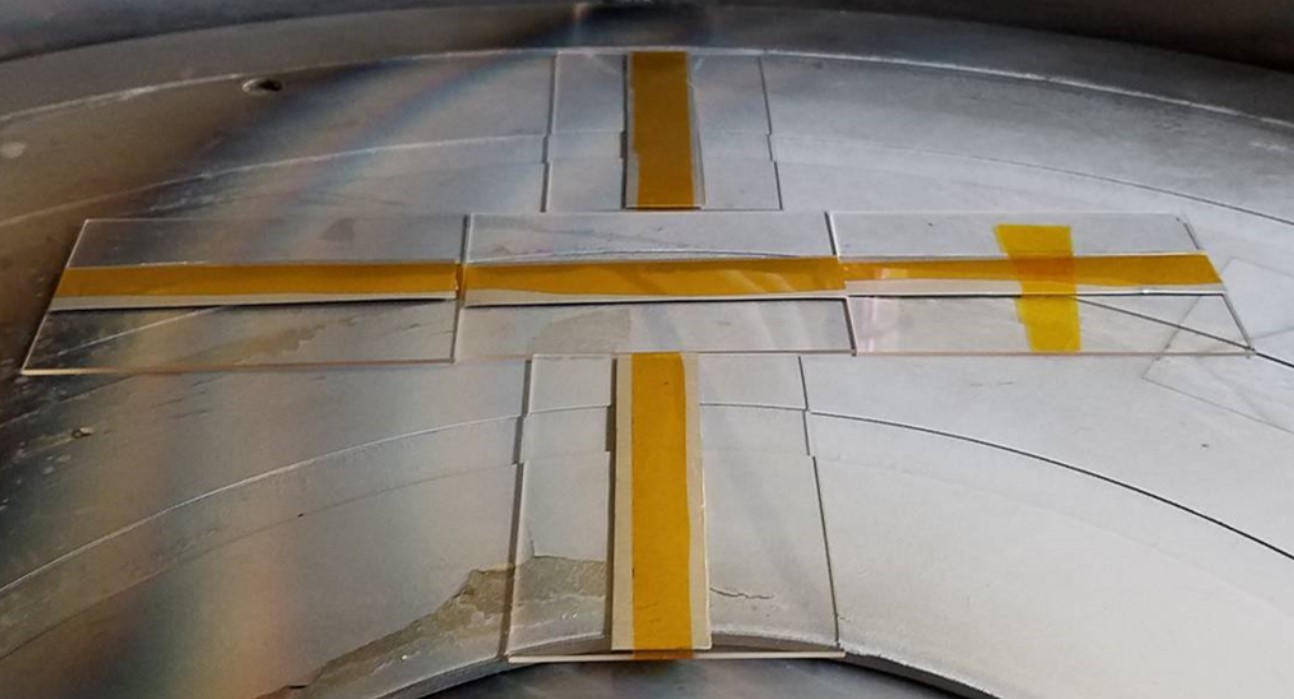
\includegraphics[width=0.5\textwidth]{tape-test-s}
\caption{Layout of tape test}
\label{fig:tape-test-s}
\end{figure}

Afterwords, the samples were removed from the sputtering machine and the tape was peeled off leaving a portion of the slide untouched by the deposition.
A machine called the Alpha-Step Profiler was used to measure the thickness of the deposited layer.
The profiler works by running a needle a predefined length across the surface.
Then it is possible to go from the clean layer to the AGe and measure the step up and thus thickness of the deposited layer.
Figure \ref{fig:surface-prof} shows a plot of the thickness measured across the samples.
\begin{figure}[htpb]
\centering
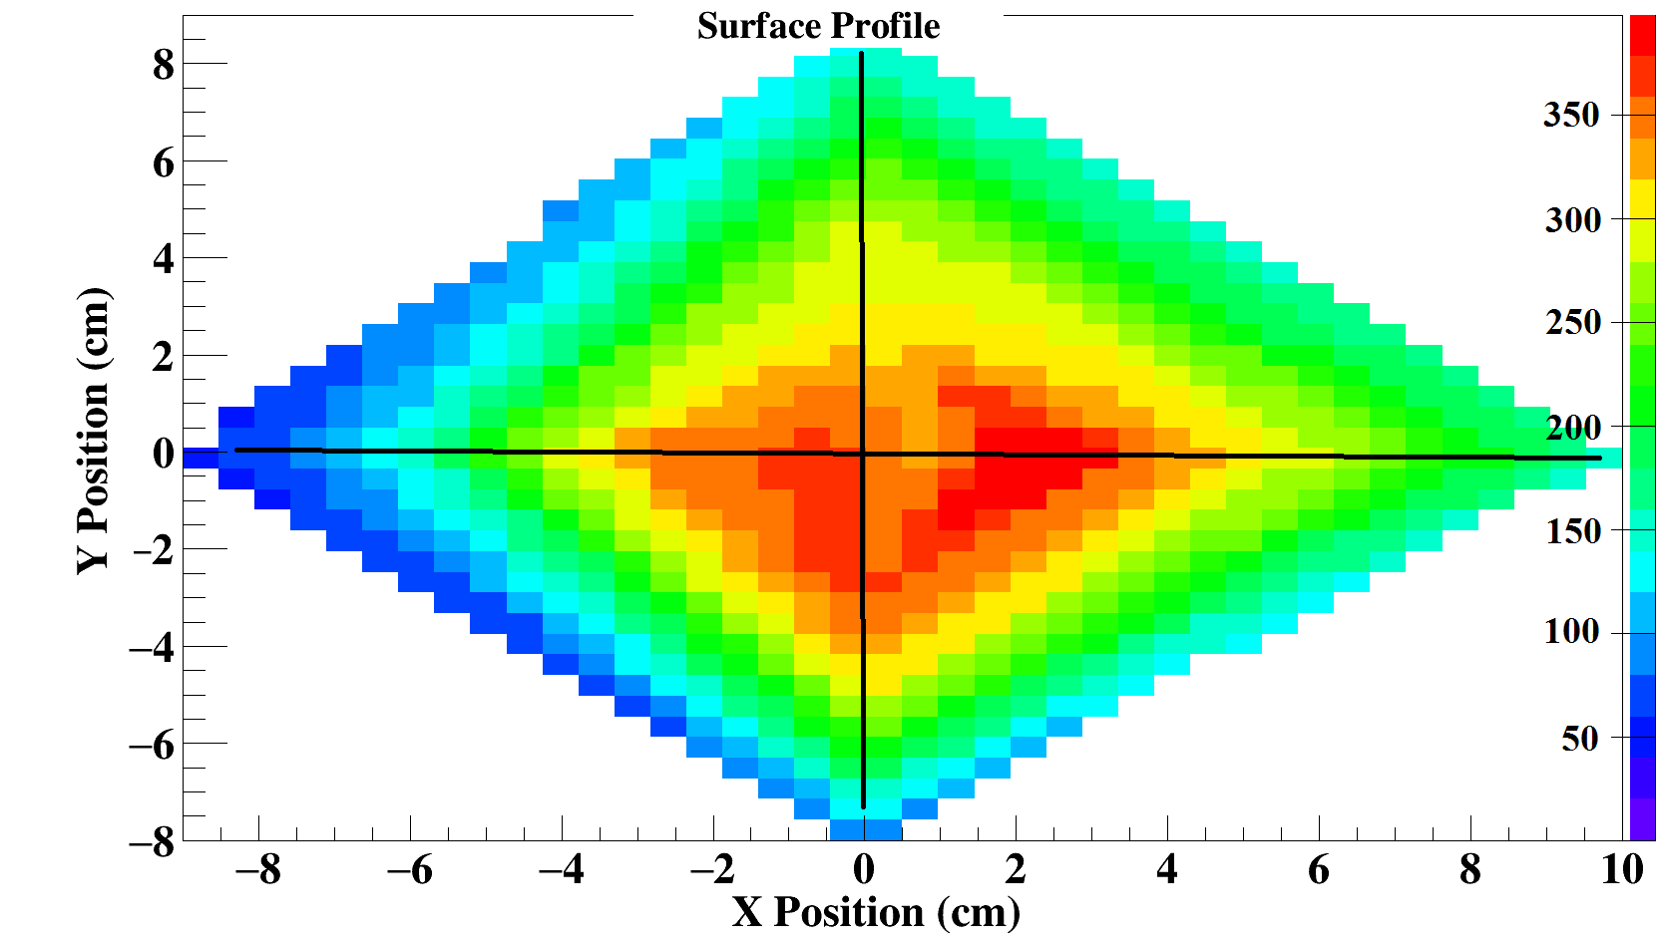
\includegraphics[width=0.8\textwidth]{surface-prof}
\caption{results of surface scan}
\label{fig:surface-prof}
\end{figure}

\subsection{Operating Procedure}
The sputtering machine at USD is a Perkin-Elmer 4400 Sputtering System.

The operating procedure for the sputtering machine is complex and care is required to make sure the system maintains working order.
It is a complex system with multiple valves, controls, power supplies, vacuum systems, and pressure monitors that all work in conjunction to deposit a thin layer of amorphous germanium on the detector sample.
One key component of the system is a cryopump that uses pressurized helium gas to quickly vacuum the system to the proper pressure.
The cryopump system can be seen in Figure ~\ref{fig:sput-flow} as blue boxes with labels connected by green lines.
The green lines exchange the helium between the cold head connected to the vacuum chamber and the compressor located in the pump room.
Before the sputtering procedure can begin, the cryopump must be turned on to allow the cold head to cool from room temperature to approximately 20K.
Prior to cooling down the cryopump, it must be vacuumed to below 100 mTorr using the rough pump describe later.
In order to vacuum the cryopump, open the foreline valve shown as E in ~\ref{fig:sput-flow}; close the valve before turning on the cryopump.
The on/off switch for the compressor is located on the panel with the other valve toggles and is labeled as "HY-VAC PUMP"

Once the cryopump is cooled down to the proper temperature, the sputtering procedure can begin.
As seen in Figure ~\ref{fig:sput-flow}, there are multiple valves for opening and closing various gas and vacuum lines.
These valves are all pneumatically opened and closed so they require a constant supply of pressurized air at 60 psi.
This pressurized air is supplied by a large Kaeser SX 5 compressor located in the pump room and shown in Figure ~\ref{fig:comp-air}.
\begin{figure}[htpb]
\centering
\includegraphics[width=\textwidth]{comp-air}
\caption{Kaeser SX 5 compressor}
\label{fig:comp-air}
\end{figure}
The compressor is turned on or off by pressing the green or red button on the control interface shown on the top left side of the figure.
Once turned on, it will automatically increase in pressure until it reaches a set point around 100 psi.
The pressure out is then reduced or increased by adjusting the pressure regulator shown on the bottom left.
It is important to check the pressure often to make sure that it is sufficiently high for if it drops too low, valves will return to the default closed position.

Once the system has been supplied with pressurized air, the valves can be opened or closed and the system is ready to be operated.
The next step is to load the detector sample into the sputtering machine and prepare for deposition.
The sputtering system should always be kept under vacuum so before it can be opened it must be returned to standard atmospheric pressure.
This is done by opening the vent valve and filling the chamber with dry nitrogen.
The toggle switch for the vent valve is located at 'A' in Figure ~\ref{fig:sput-flow}.
The nitrogen in routed in from a tank located in a separate room behind the pump room and is kept at approximately 10 to 15 psi.

After the chamber has returned to atmospheric pressure it can be opened using a hydraulic lift system that is powered through the RF power generator.
The sample can now be carefully placed inside the chamber centering it under the amorphous germanium target as seen in Figure ~\ref{fig:sput-open}.
\begin{figure}[htpb]
\centering
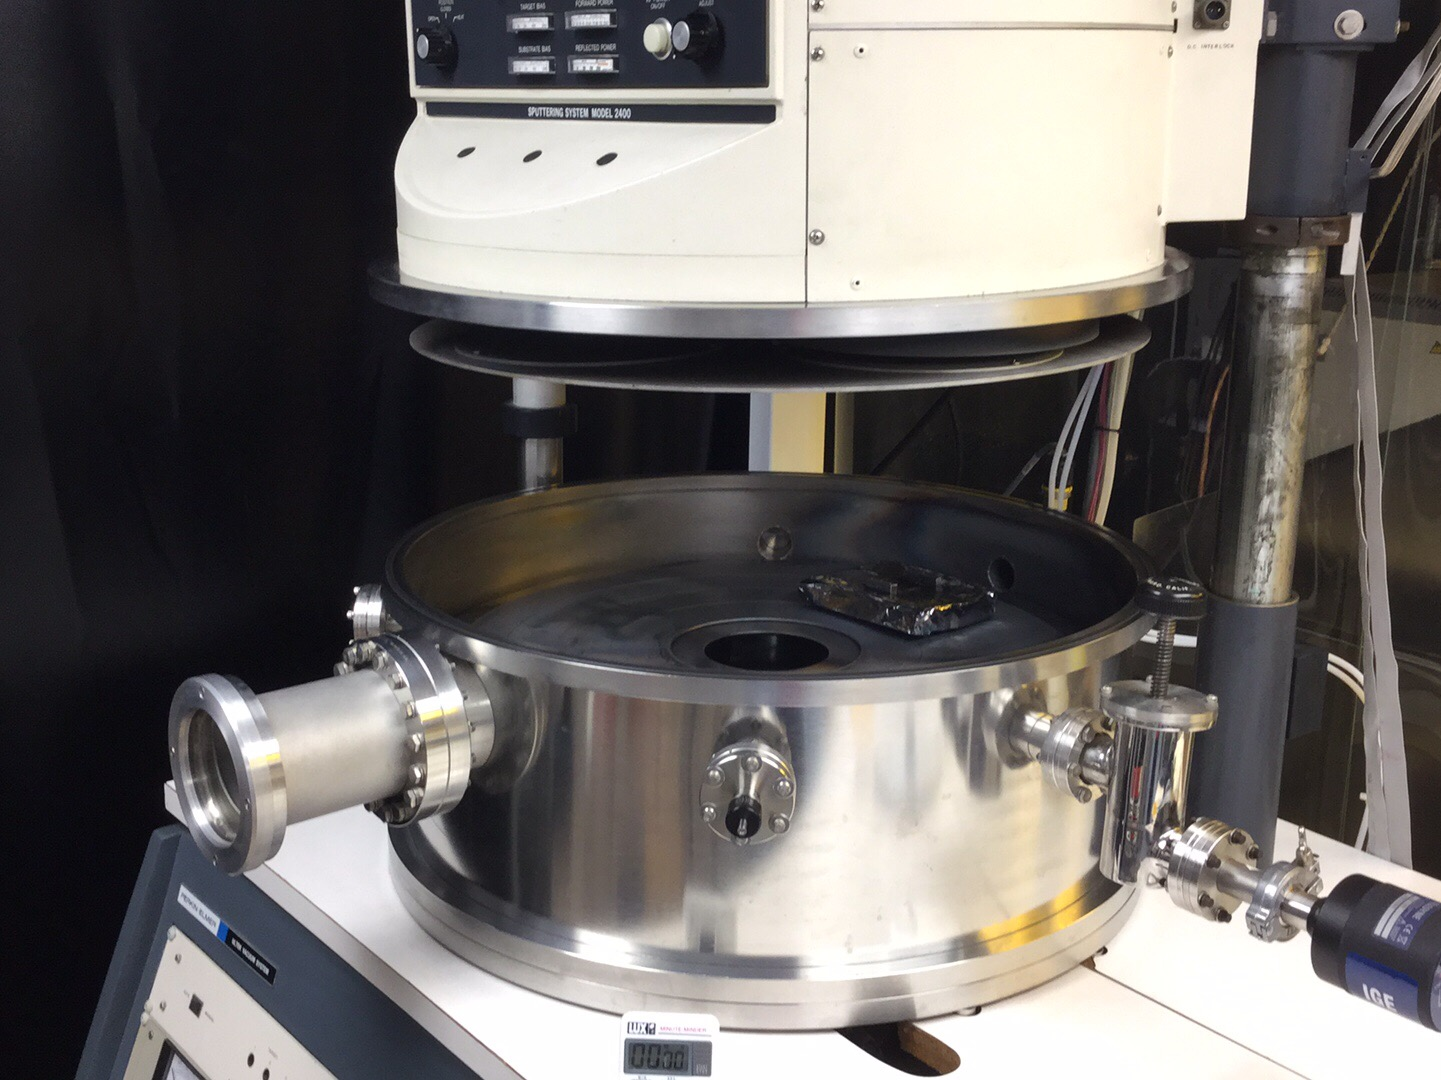
\includegraphics[width=0.6\textwidth]{sput-open}
\caption{Sputtering machine with chamber open}
\label{fig:sput-open}
\end{figure}
A jig is used to hold the detectors by the wings during the sputtering process.
It is designed to be adjustable, allowing for various detector sizes and geometries.
After the detector sample has been chemically etched it can be loaded onto the jig and then into the sputtering machine.

Once the sample is loaded the chamber can be closed and vacuum pumping can begin.
The first stage of pumping is done by a rough pump which takes the chamber from atmospheric pressure down to below 100 mTorr.
The rough pump is turned on or off by switching an electrical breaker located outside of the clean room.
After the pump is on and running normally, the roughing valve can be opened.
Opening the roughing valve allows the rough pump to vacuum the chamber from atmospheric pressure to around 100 mTorr.

\begin{sidewaysfigure}
\includegraphics[width=\textwidth]{sput-flow}
\caption{This is a diagram of the Sputtering machine vacuum and gas system. Each valve is connected to a pressurized air line.}
\label{fig:sput-flow}
\end{sidewaysfigure}

Once the chamber has reached some pressure between 50-100 mTorr the roughing valve can be closed and the HY-VAC VALVE, shown as D in Figure \ref{fig:sput-flow}, can be opened.
The cryopump will then be able to vacuum the system to the required $10^{-6}$ Torr for sputtering.
The sputtering machine takes less than five minutes to go from atmosphere to $10^{-3}$ Torr using the rough pump and a further 2-3 hours to reach $10^{-6}$ Torr using the cryopump.

After proper vacuum pressure is achieved the sputtering deposition procedure can start.
The first thing is to start the water chiller and make sure the proper lines are selected.
The chiller is used to provide cooling to the target and stage during deposition as the plasma generates considerable heat.
It is located in the pump room and is show in Figure ~\ref{fig:water-cool}.
The middle picture of the figure shows the side view of the chiller where the separate lines to the sputtering and e-beam machines are visible.
The selection of lines is done by switching two valves on the back of the water chiller.
The handles of the valves indicate the direction of flow and is used to determine which line is selected.
\begin{figure}[htpb]
\centering
\includegraphics[width=\textwidth]{water-cool}
\caption{Water chiller for cooling the sputtering machine and e-beam evaporator}
\label{fig:water-cool}
\end{figure}

Once the water chiller has reached the set point temperature of \SI{10}{\celsius}, the deposition can start.
First the RF power supply should be turned on by flipping the switch at the base of the front.
The throttle valve, shown as C in Figure ~\ref{fig:sput-flow}, can now be turned on to limit the vacuuming of the chamber.
Now the mixed gas can be vented into the chamber using the gas flow adjuster show in the figure.
To the left of the flow controller is the toggle switch to open the mixed gas line.
Then, the flow controller is turned on and set to approximately 50 SCCM.
Due to the throttle valve being on, the chamber will begin to increase in pressure based on the flow controller setting.
The key is to adjust the flow rate until a steady 14 mTorr chamber pressure is achieved.

After the chamber has stabilized at 14 mTorr the RF power can be introduced to the gas in order to generate the plasma required for sputtering.
This is done by pressing the power on button at the top of the chamber show in Figure.
The power can then slowly be increased to the marked point.
During this increase in power, the tune and load must be adjusted to keep the reflected power to a minimum and make sure all the power is transferred into the gas.
At a certain point, the plasma will form and the reading for forward and reflected power will jump up.
It is again necessary to quickly readjust the tune and load to get the reflected power back to 0.
After the reflected power is reduced, the power can be further adjusted to the required level, usually around 100 watts.
Once the plasma is generated, the user must wait for at least five minutes with the shutter closed to bombard the target and clean off the outer layer.
After this five minutes the shutter can be opened which will start deposition on the sample.
The machine can then be run for 15 minutes with the shutter open.
After 15 minutes have elapsed, the RF power can be turned off.
The detector sample should have accumulated a layer of amorphous germanium that is around 300 nm thick.

The machine can then be opened up and the sample flipped over to coat the other side.
This is done by first turning down the flow rate of the mixed gas to zero and closing the valve.
Then the throttle valve can be turned off followed by closing the HY-VAC VALVE.
At this point the chamber should no longer be pumping so the vent valve can be opened and the chamber returned to atmospheric pressure.
The sample can then be flipped and the sputtering process starts again with closing the chamber and rough pumping.

%}}}
% Section: Aluminum deposition%{{{

\section{Aluminum Deposition}
\subsection{Principles of e-beam}
Electron-beam deposition is a method of thin film deposition where a target metal is bombarded with an electron beam given off by a tungsten filament.
The electron beam then causes the atoms to transform into the gaseous phase which coats and solidifies onto everything within line of site of the material.
In order for e-beam deposition to work, the chamber must also be kept under high vacuum to make sure the electrons can make it from the gun to the crucible without interference.
\begin{figure}[htpb]
\centering
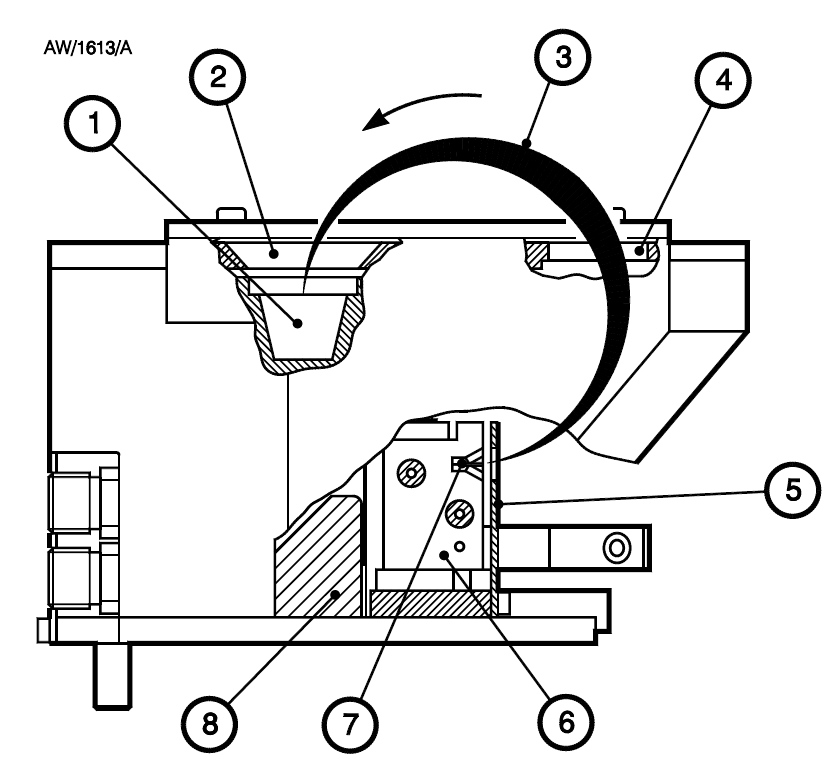
\includegraphics[width=0.7\textwidth]{ebeam-diagram}
\caption{Cutaway drawing of the ebeam mechanics}
\label{fig:ebeam-diagram}
\end{figure}

\subsection{E-Beam Calibration}
The calibration of the e-beam was similar to the sputtering machine with a key difference being that the target location for the sample is fixed.
Due to this, only one glass slide was needed to get a good profile of the deposition thickness.
Another difference from the sputtering machine is that the e-beam has a deposition rate and thickness monitor.
Thus the accuracy of the monitor was also verified in the test.

Figure \ref{fig:tape-test-e} shows the glass slide after aluminum deposition.
Figure \ref{fig:alpha-step-e} shows a plot of thickness vs distance generated by the alpha step profiler.
In it, the step from an area with aluminum to one without is clearly visible.

\begin{table}[htpb]
\centering
\begin{tabular}{ |p{4cm}|p{4cm}|p{4cm}|  }
 \hline
 \multicolumn{3}{|c|}{E-Beam deposition profile} \\
 \hline
 Test (\#)&Step Thickness (nm)&Percent Difference (\%)\\
 \hline
 1   & 268.7    &7.48\\
 2&   256.7  & 2.68\\
 3 &268.1 & 7.24\\
 4    &246.2 & 1.52\\
 \hline
\end{tabular}
\caption{Table listing data gathered from alpha profiler}
\label{table:test-e}
\end{table}

\begin{figure}[htpb]
\centering

\includegraphics[width=0.5\textwidth]{tape-test-e}
\caption{E-Beam tape test}
\label{fig:tape-test-e}
\end{figure}

\begin{figure}[htpb]
\centering
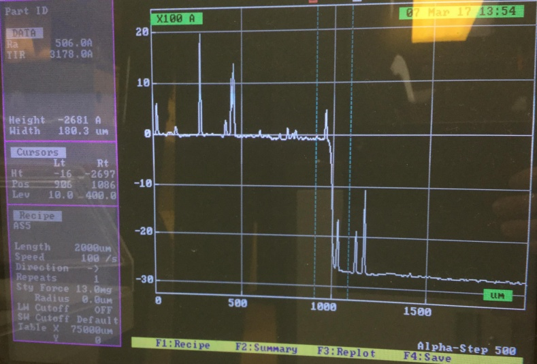
\includegraphics[width=0.7\textwidth]{alpha-step-e}
\caption{Surface profile for ebeam}
\label{fig:alpha-step-e}
\end{figure}

\subsection{Operating Procedure}
Once the detector sample has been completely coated with a layer of amorphous germanium, aluminum can be deposited on the top and bottom surface to create the electrical contacts.
The aluminum serves as the electrical contact and covers the entire surface of the top and bottom which is what defines the detector as planar.

The e-beam has two separate power supplies: one for powering the controls and vacuum system, and another for supplying the high voltage to the electron gun.
To initiate the startup procedure, the control power supply is turned on.
Afterwords the controls can be activated by switching the selector from 0 to 1 as seen in Figure \ref{fig:vac-control}.
This will supply power to the vacuum system which needs to be activated by following the prompts on the screen.
Pressing start will initialize the system, activating the rough and turbo pump.
Once the turbo pump has reached 42 krpm it is ready to vacuum.
\begin{figure}[htpb]
\centering
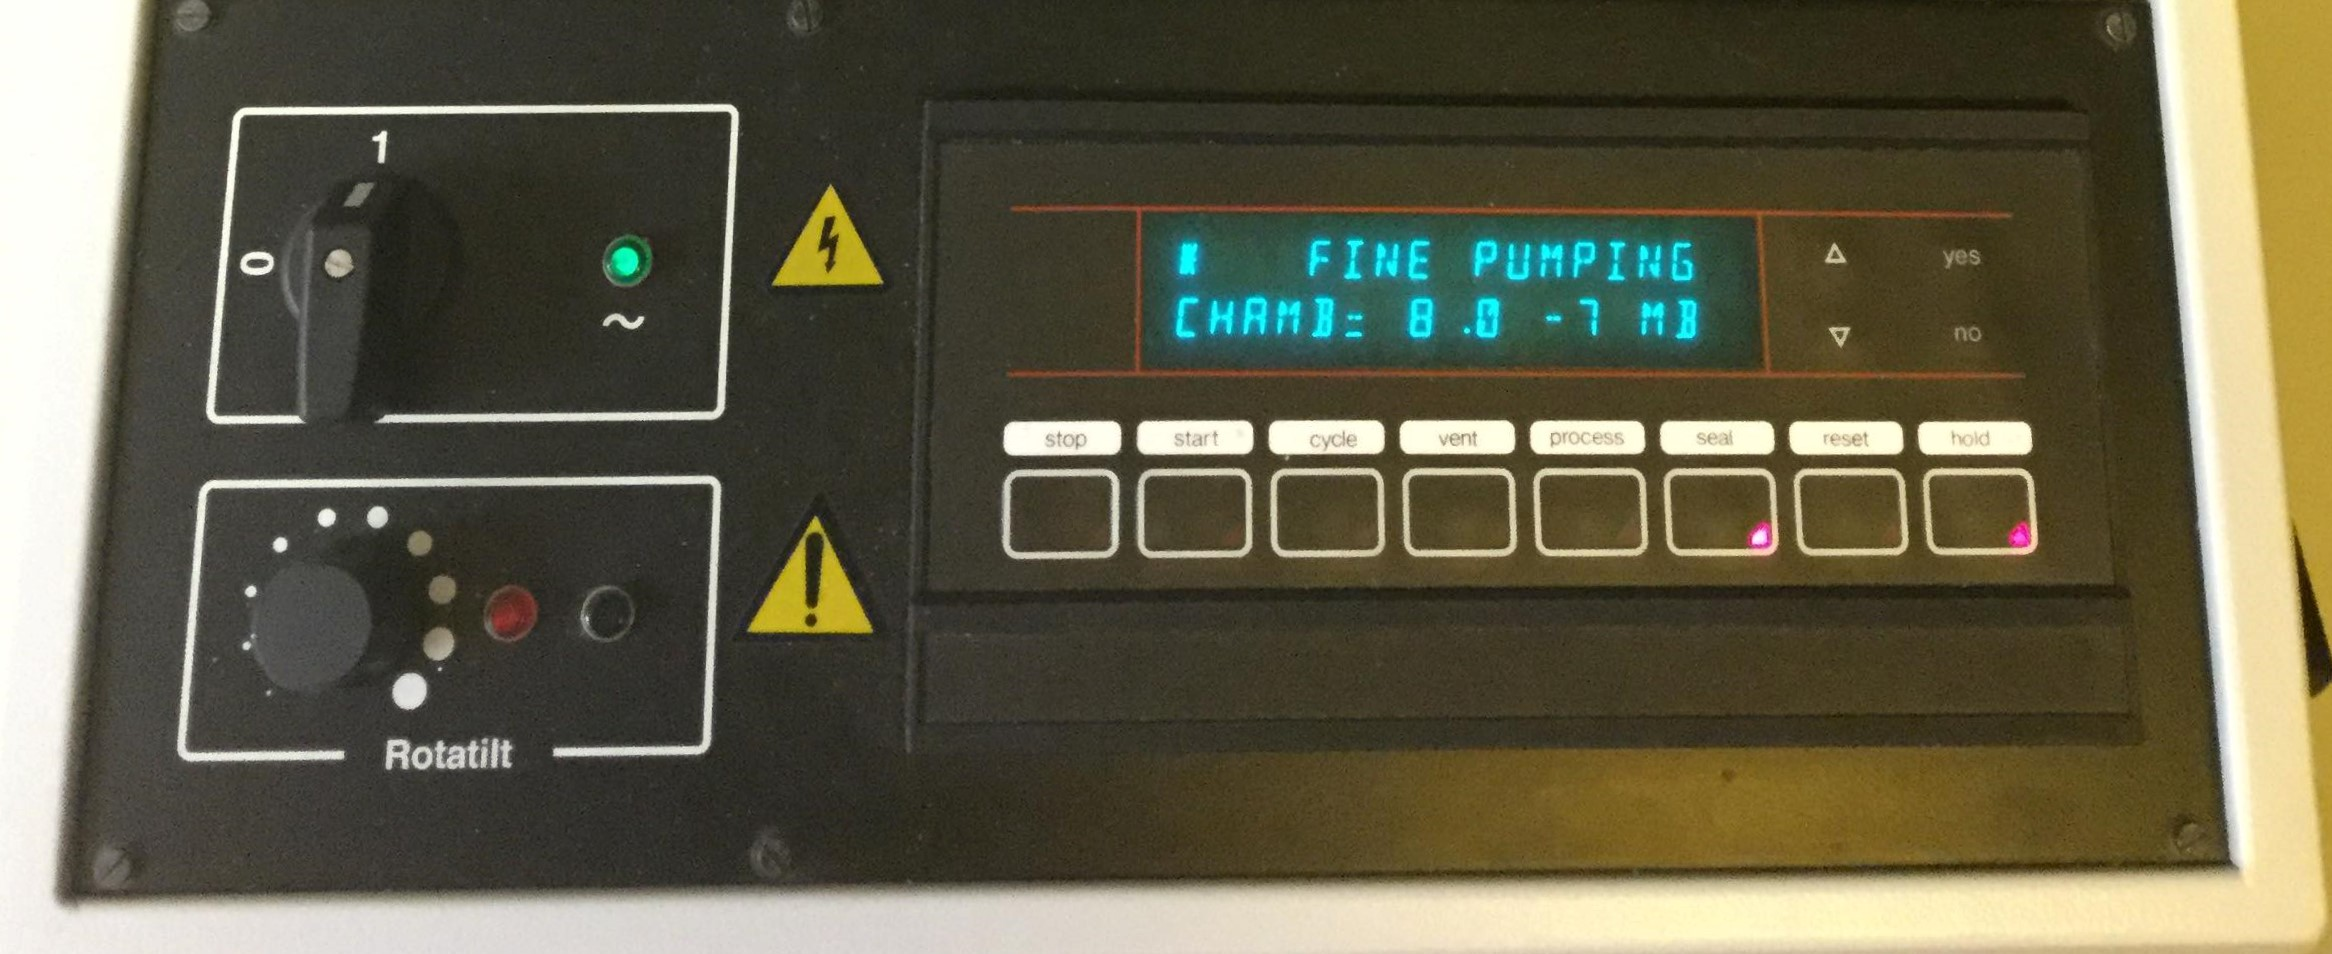
\includegraphics[width=\textwidth]{vac-control}
\caption{E-Beam vacuum controls and power switch}
\label{fig:vac-control}
\end{figure}

The vacuum pumps are located in a cabinet directly under the e-beam chamber as shown in Figure \ref{fig:ebeam-flow}.
The turbo pump has a separate controller that displays the speed which can be seen when the cabinet is opened.
Pressing seal will isolate the turbo pump from the chamber and allow it to be vented so the sample can be placed inside.
Once sealed, the vent button can be pressed which will open the valve allowing nitrogen to fill the chamber.
After the chamber has reached atmospheric pressure the door will be able to open and the sample can be placed loaded onto the holder shown in Figure \ref{fig:ebeam-holder}.
The holder can then be secured inside the chamber using a hex screw and wrench.
\begin{figure}[htpb]
\centering
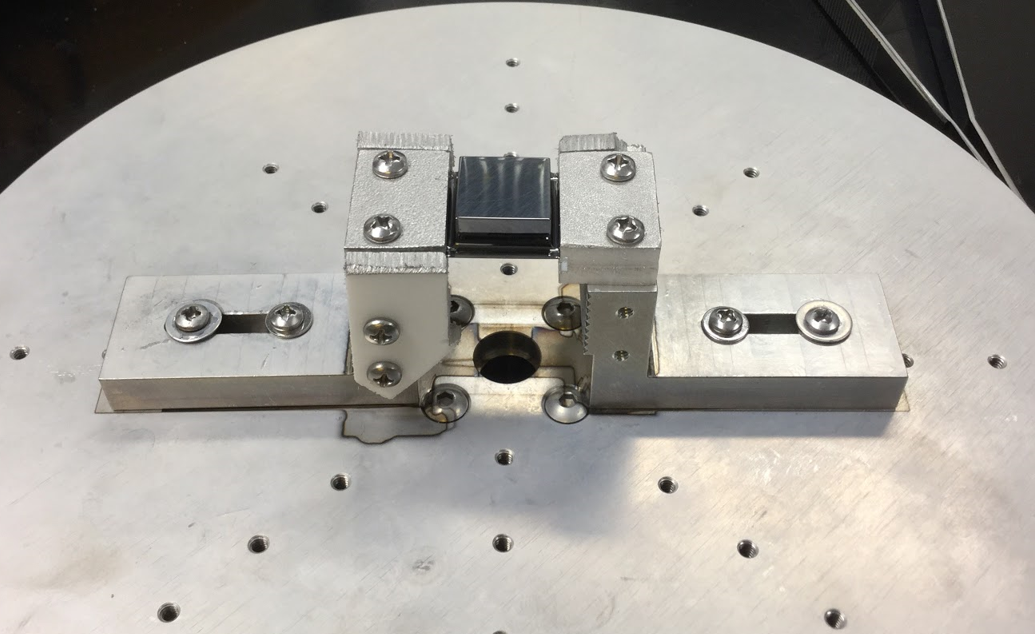
\includegraphics[width=0.6\textwidth]{ebeam-holder}
\caption{Sample holder for the E-Beam}
\label{fig:ebeam-holder}
\end{figure}
Once the sample is loaded, the chamber door can be closed and the process button pressed.
This will open up the chamber to the vacuum system and start the rough pump.
Once the vacuum has reached sufficient level, the turbo pump will automatically turn on.
The vacuum must reach around $10^{-6}$ torr before the aluminum deposition can start.

Once the proper pressure is reached, the aluminum deposition can begin.
To start, the electron gun power supply is turned on by flipping the switch on the front panel of the high voltage power supply.
Then the on/off switch on the source control, shown in the upper right of Figure \ref{fig:source-control}, can be switched on.
The gun button can then be depressed.
This will provide around 4.9 kV to the electron gun, however, the current remains at 0 so there is no flow of electrons yet.
The current can then be turned up slowly using the dial labeled current.
\begin{figure}[htpb]
\centering
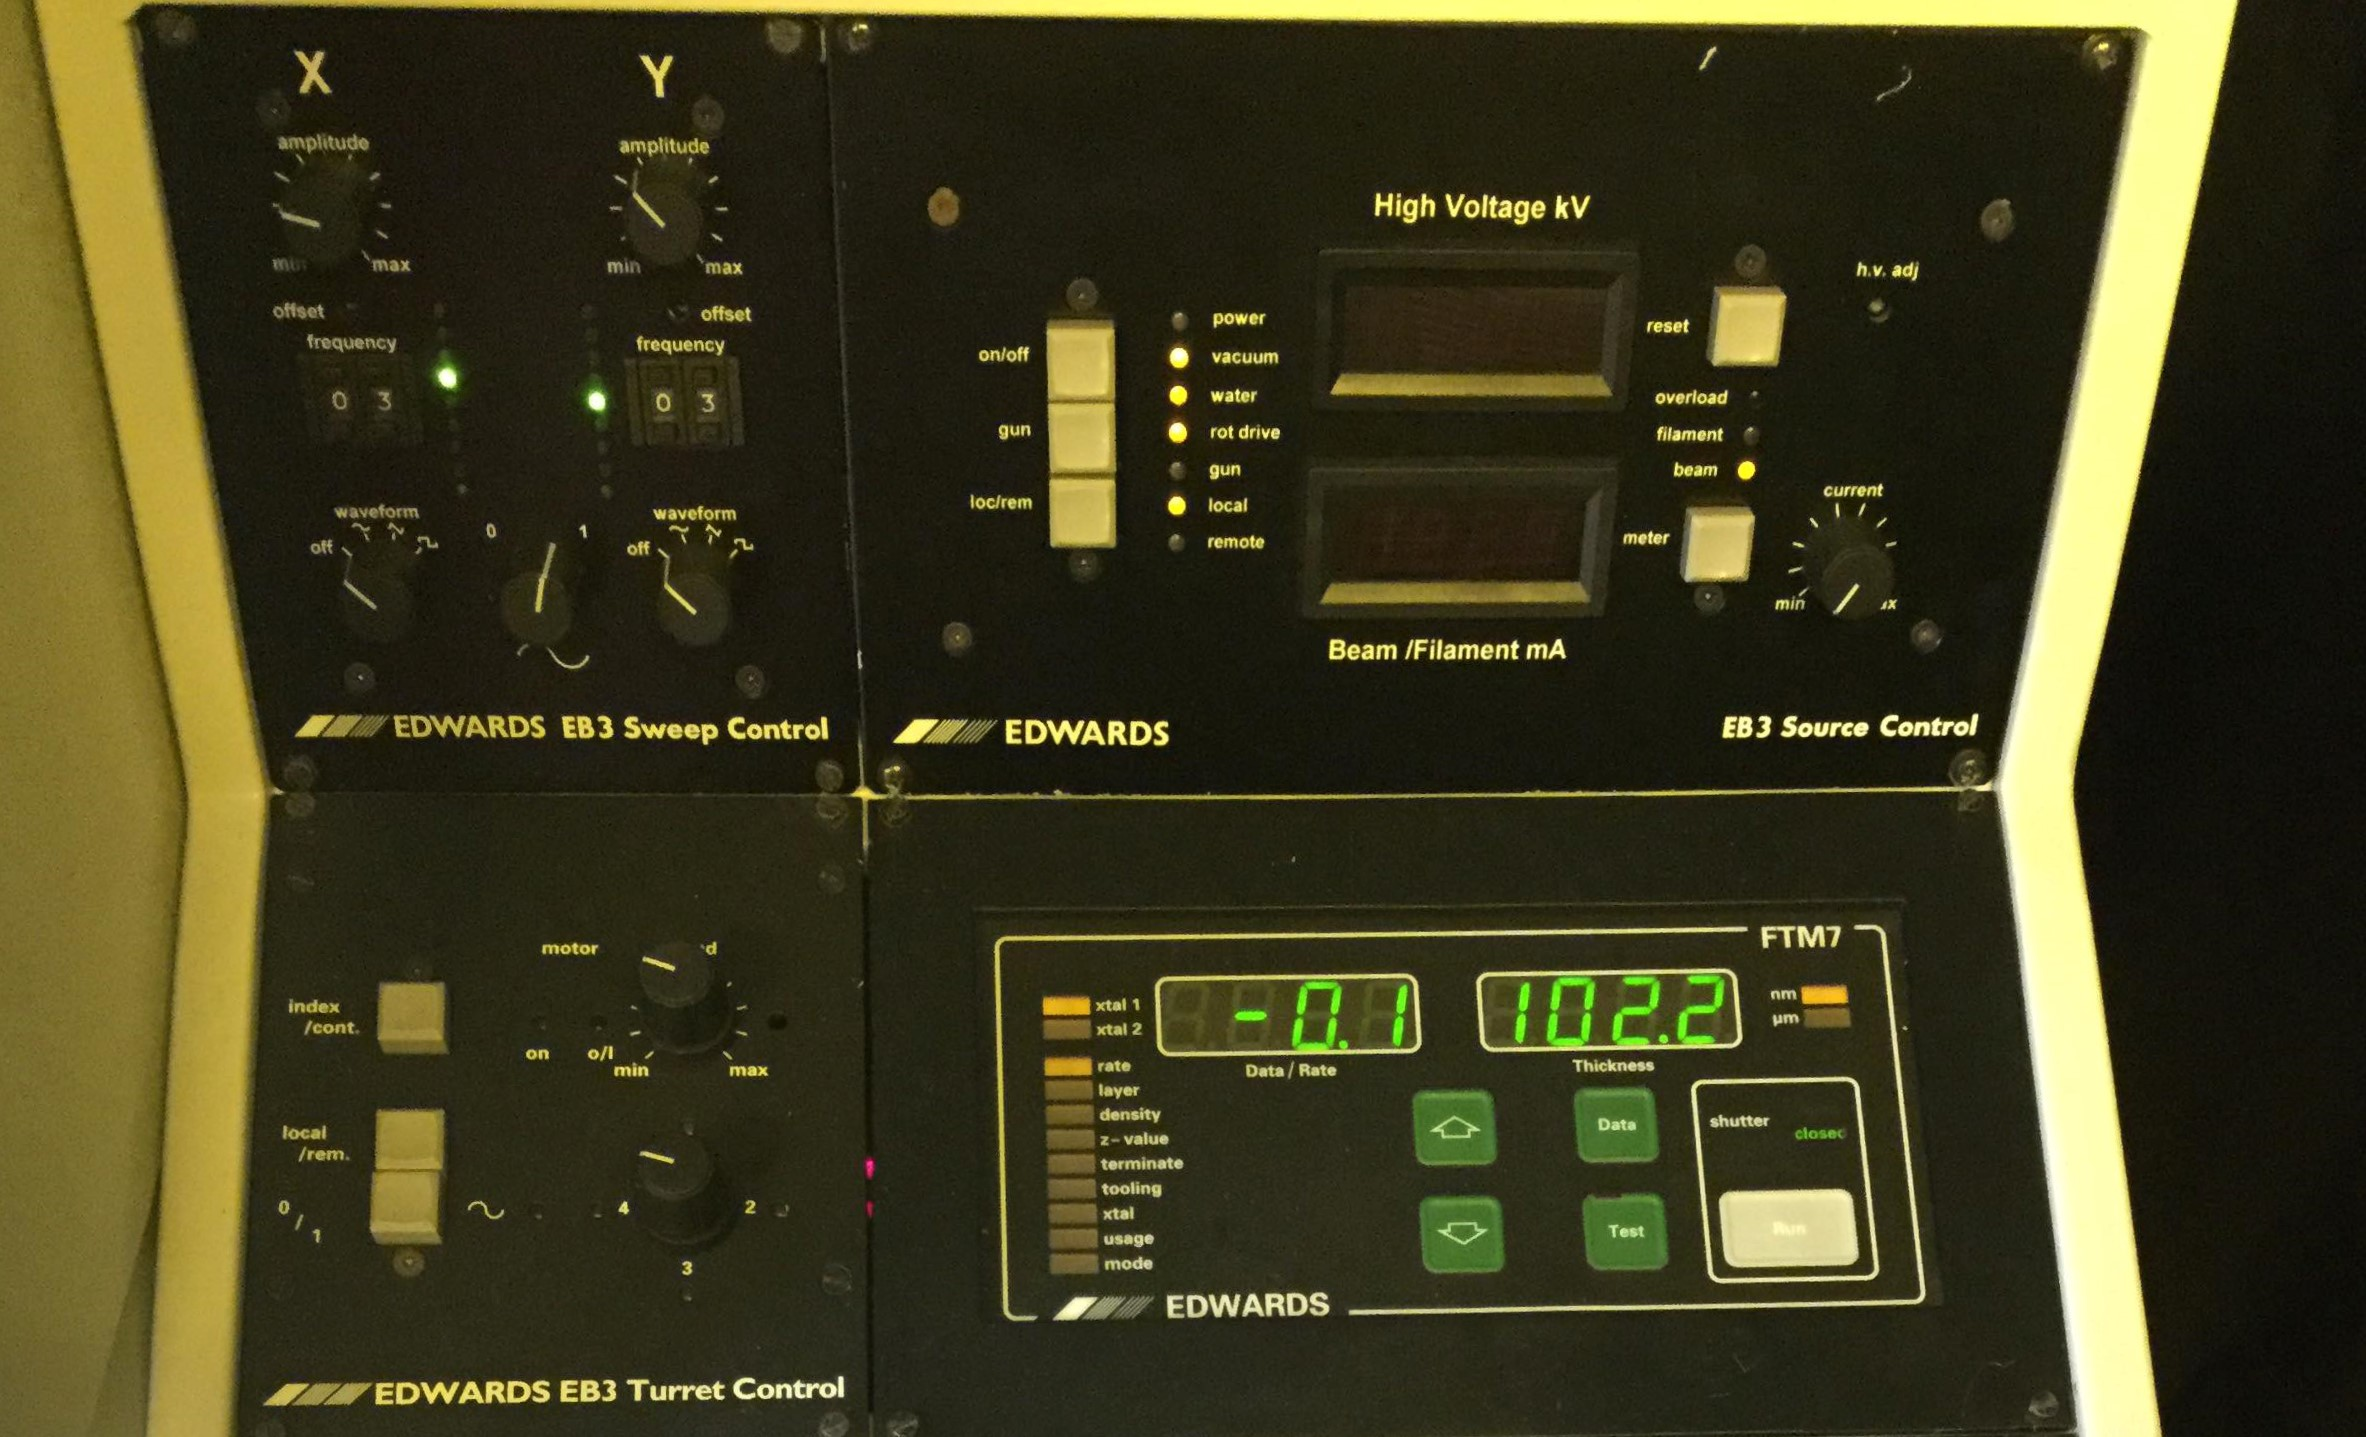
\includegraphics[width=\textwidth]{source-control}
\caption{E-Beam controls for the electron gun, sweep, crystal monitor, and crucible select}
\label{fig:source-control}
\end{figure}

Once the current has reached around 17 mA, the sweep control can be turned on by switching the dial from 0 to 1.
The current can then be continued to increase until the Data/Rate of the crystal monitor is a steady 0.1-0.2 nm/min.
Once the deposition has stabilized, the shutter can be opened by pressing run on the FTM7 control panel.
This will automatically open the shutter until the predefined thickness, usually around 100nm, is reached.
The shutter will then automatically close and the current can slowly be reduced to zero.

\begin{sidewaysfigure}
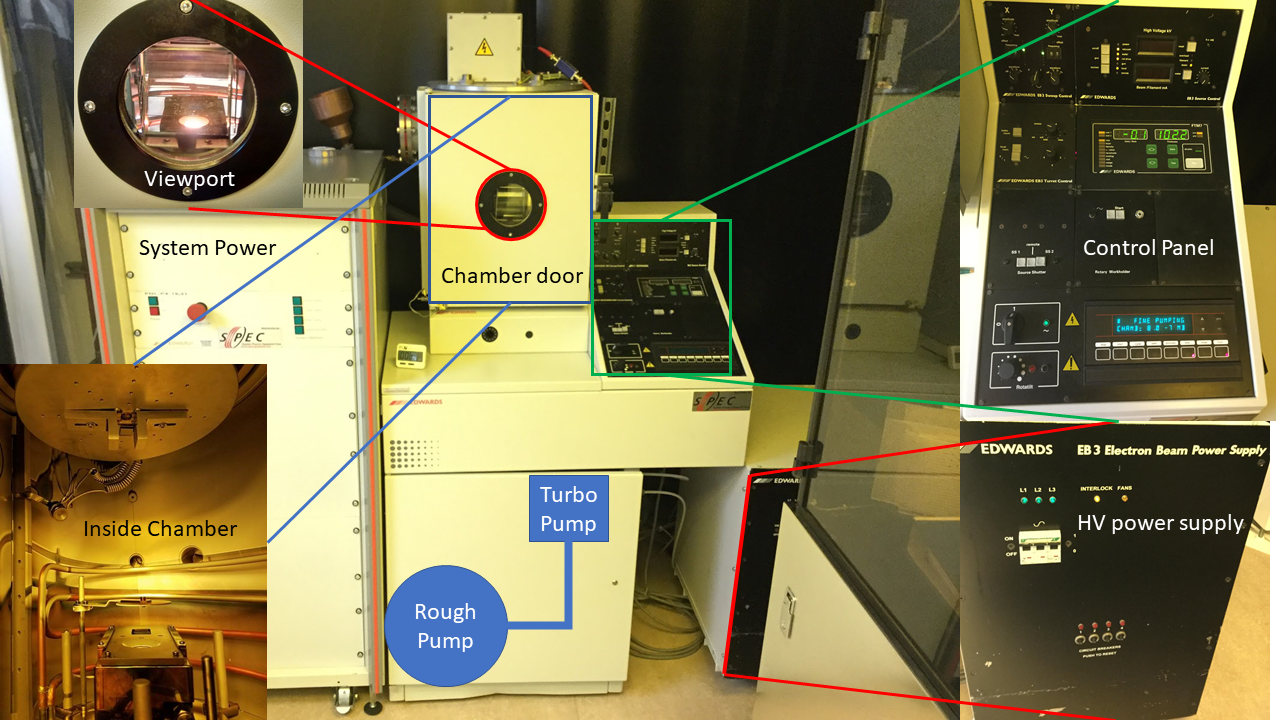
\includegraphics[width=\textwidth]{ebeam-flow}
\caption{This is a diagram of the of the electron beam machine.It is used to deposit aluminum onto the detector sample.}
\label{fig:ebeam-flow}
\end{sidewaysfigure}
%}}}
% Section: Final Steps%{{{

\section{Final Steps}
The nature of e-beam deposition usually leaves the entire chamber coated with aluminum, including the side surface of the detector sample.
While aluminum is great for the contacts, it can cause the detector to breakdown if any is left on the surfaces other than the contacts.
Thus after aluminum deposition, the sides must be etched with acid to remove any aluminum before the detector can be tested.
However, this etch must not attack any of the aluminum left over on the surface.
To prevent this from happening, a mask of tape is placed over the top and bottom surfaces before etching as seen in Figure \ref{fig:taped}.
The tape used is acid resistant and has low adhesion so that the surface will not be damaged and no residue will be left after it is removed.
\begin{figure}[htpb]
\centering
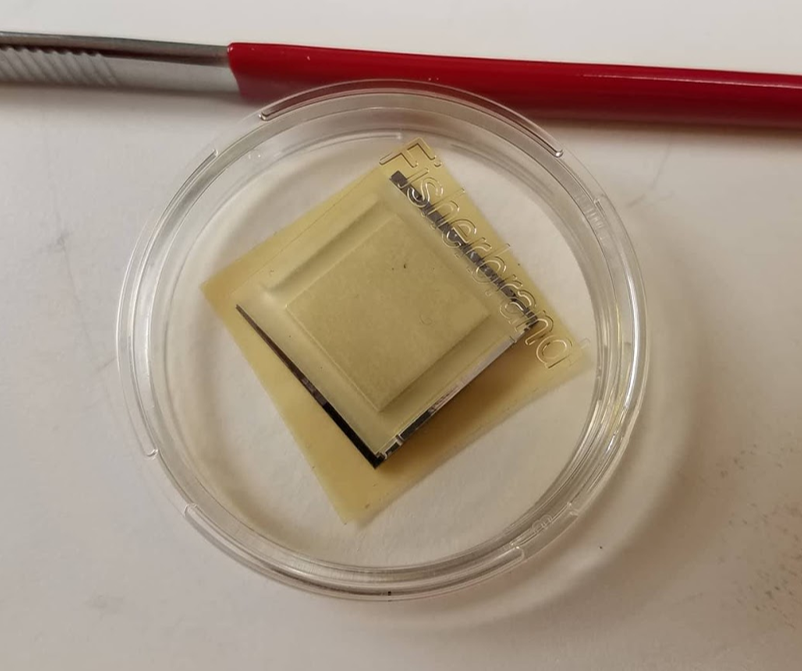
\includegraphics[width=0.5\textwidth]{taped}
\caption{Detector with tape masking before etching.}
\label{fig:taped}
\end{figure}

The taped sample is dipped in 1\% HF for a few minutes until all of the aluminum has been etched away.
The HF does not attack germanium so the amorphous germanium blocking layer beneath will be untouched.
After the aluminum is etched away, the tape is carefully removed using a Q-tip and tweezer being careful to not scratch the surface.
The detector is now complete and can be loaded into the cryostat for testing.

%}}}



%%%%%%%%%%%%%%%%
% Chapter 6
%%%%%%%%%%%%%%%%

\chapter{Detector Testing Facilities}
The last step of manufacturing is to test the electrical properties of the detector and evaluate whether it is functioning properly or not.
Several properties must be analyzed in order to determine the quality of the detector; the first of which is leakage current.
In order for the detector to work properly, it must function as a basic capacitor.
If current can flow while the detector has applied voltage, then the amorphous germanium layer is not properly blocking holes and electrons which means the detector will not function.
Thus, a measure of leakage current is a necessary initial step to analyze if the detector will work at all.

If the leakage current is tested and determined to be of an acceptable level (on the order of a few picoamps or less), testing can proceed.
The next property measured is the detector capacitance.
This measurement is made using an injected pulsar and can also determine the depletion voltage of the detector.
The detector capacitance and depletion voltage can also give an accurate measurement for the impurity concentration of the germanium.
Finally the detector spectrum is measured using several radioactive sources such as cobalt 60 and cesium 137.
From this spectrum, the energy resolution of the detector can be determined and thus the overall quality.

All of these measurement must be taken while the detector is at cryogenic temperatures as described in chapter 2.
They also require the integration of several pieces of electronics that must be easily interchanged to make the different measurements.
The cryostat used at USD is shown in Figure \ref{fig:cryostat-whole}.
In the figure, the black cords coming into the base on the right and left side are a mix of high voltage and signal cables.
The flex tube coming into the middle is a vacuum tube.
The large black cylinder on top is the chicken feeder style liquid nitrogen dewar.
The metal cylinder at the base is where the detector sits.
\begin{figure}[htpb]
\centering
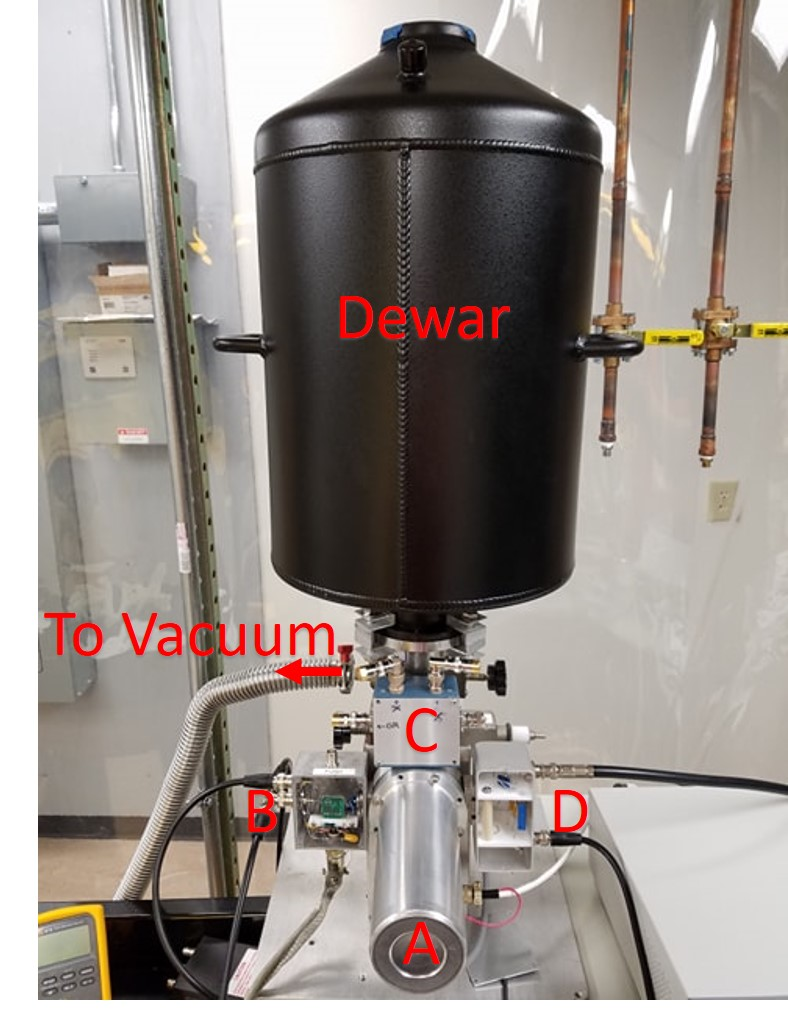
\includegraphics[width=\textwidth]{cryostat-whole}
\caption{Cryostat system used for detector calibration.}
\label{fig:cryostat-whole}
\end{figure}

\section{Cryostat}
needs to be easily cooled
measure temp and provide heat.
Key is the L shaped pipe were LN is stored along with gravity feed Dewar. This is the difference between most cryostats.
Cooling finger
Submersable 
Gravity feed
Advantages and disadvantages of these.

Have chapter- on test stand

Chapter Detector characterization
Sections- each with methods and results
Leakage current
Capacitance
Spectrum


\begin{figure}[htpb]
\centering
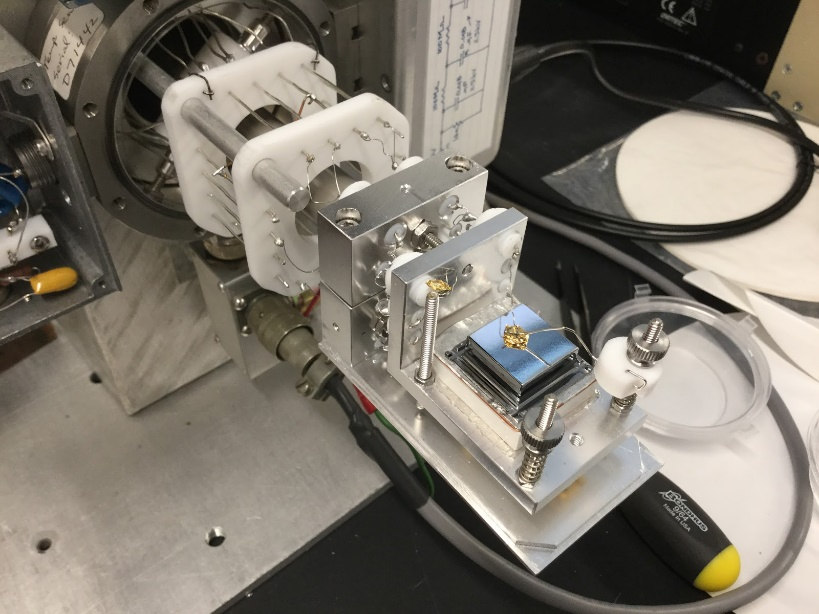
\includegraphics[width=0.8\textwidth]{inner-cryostat}
\caption{}
\label{fig:inner-cryostat}
\end{figure}

\begin{figure}[htpb]
\centering
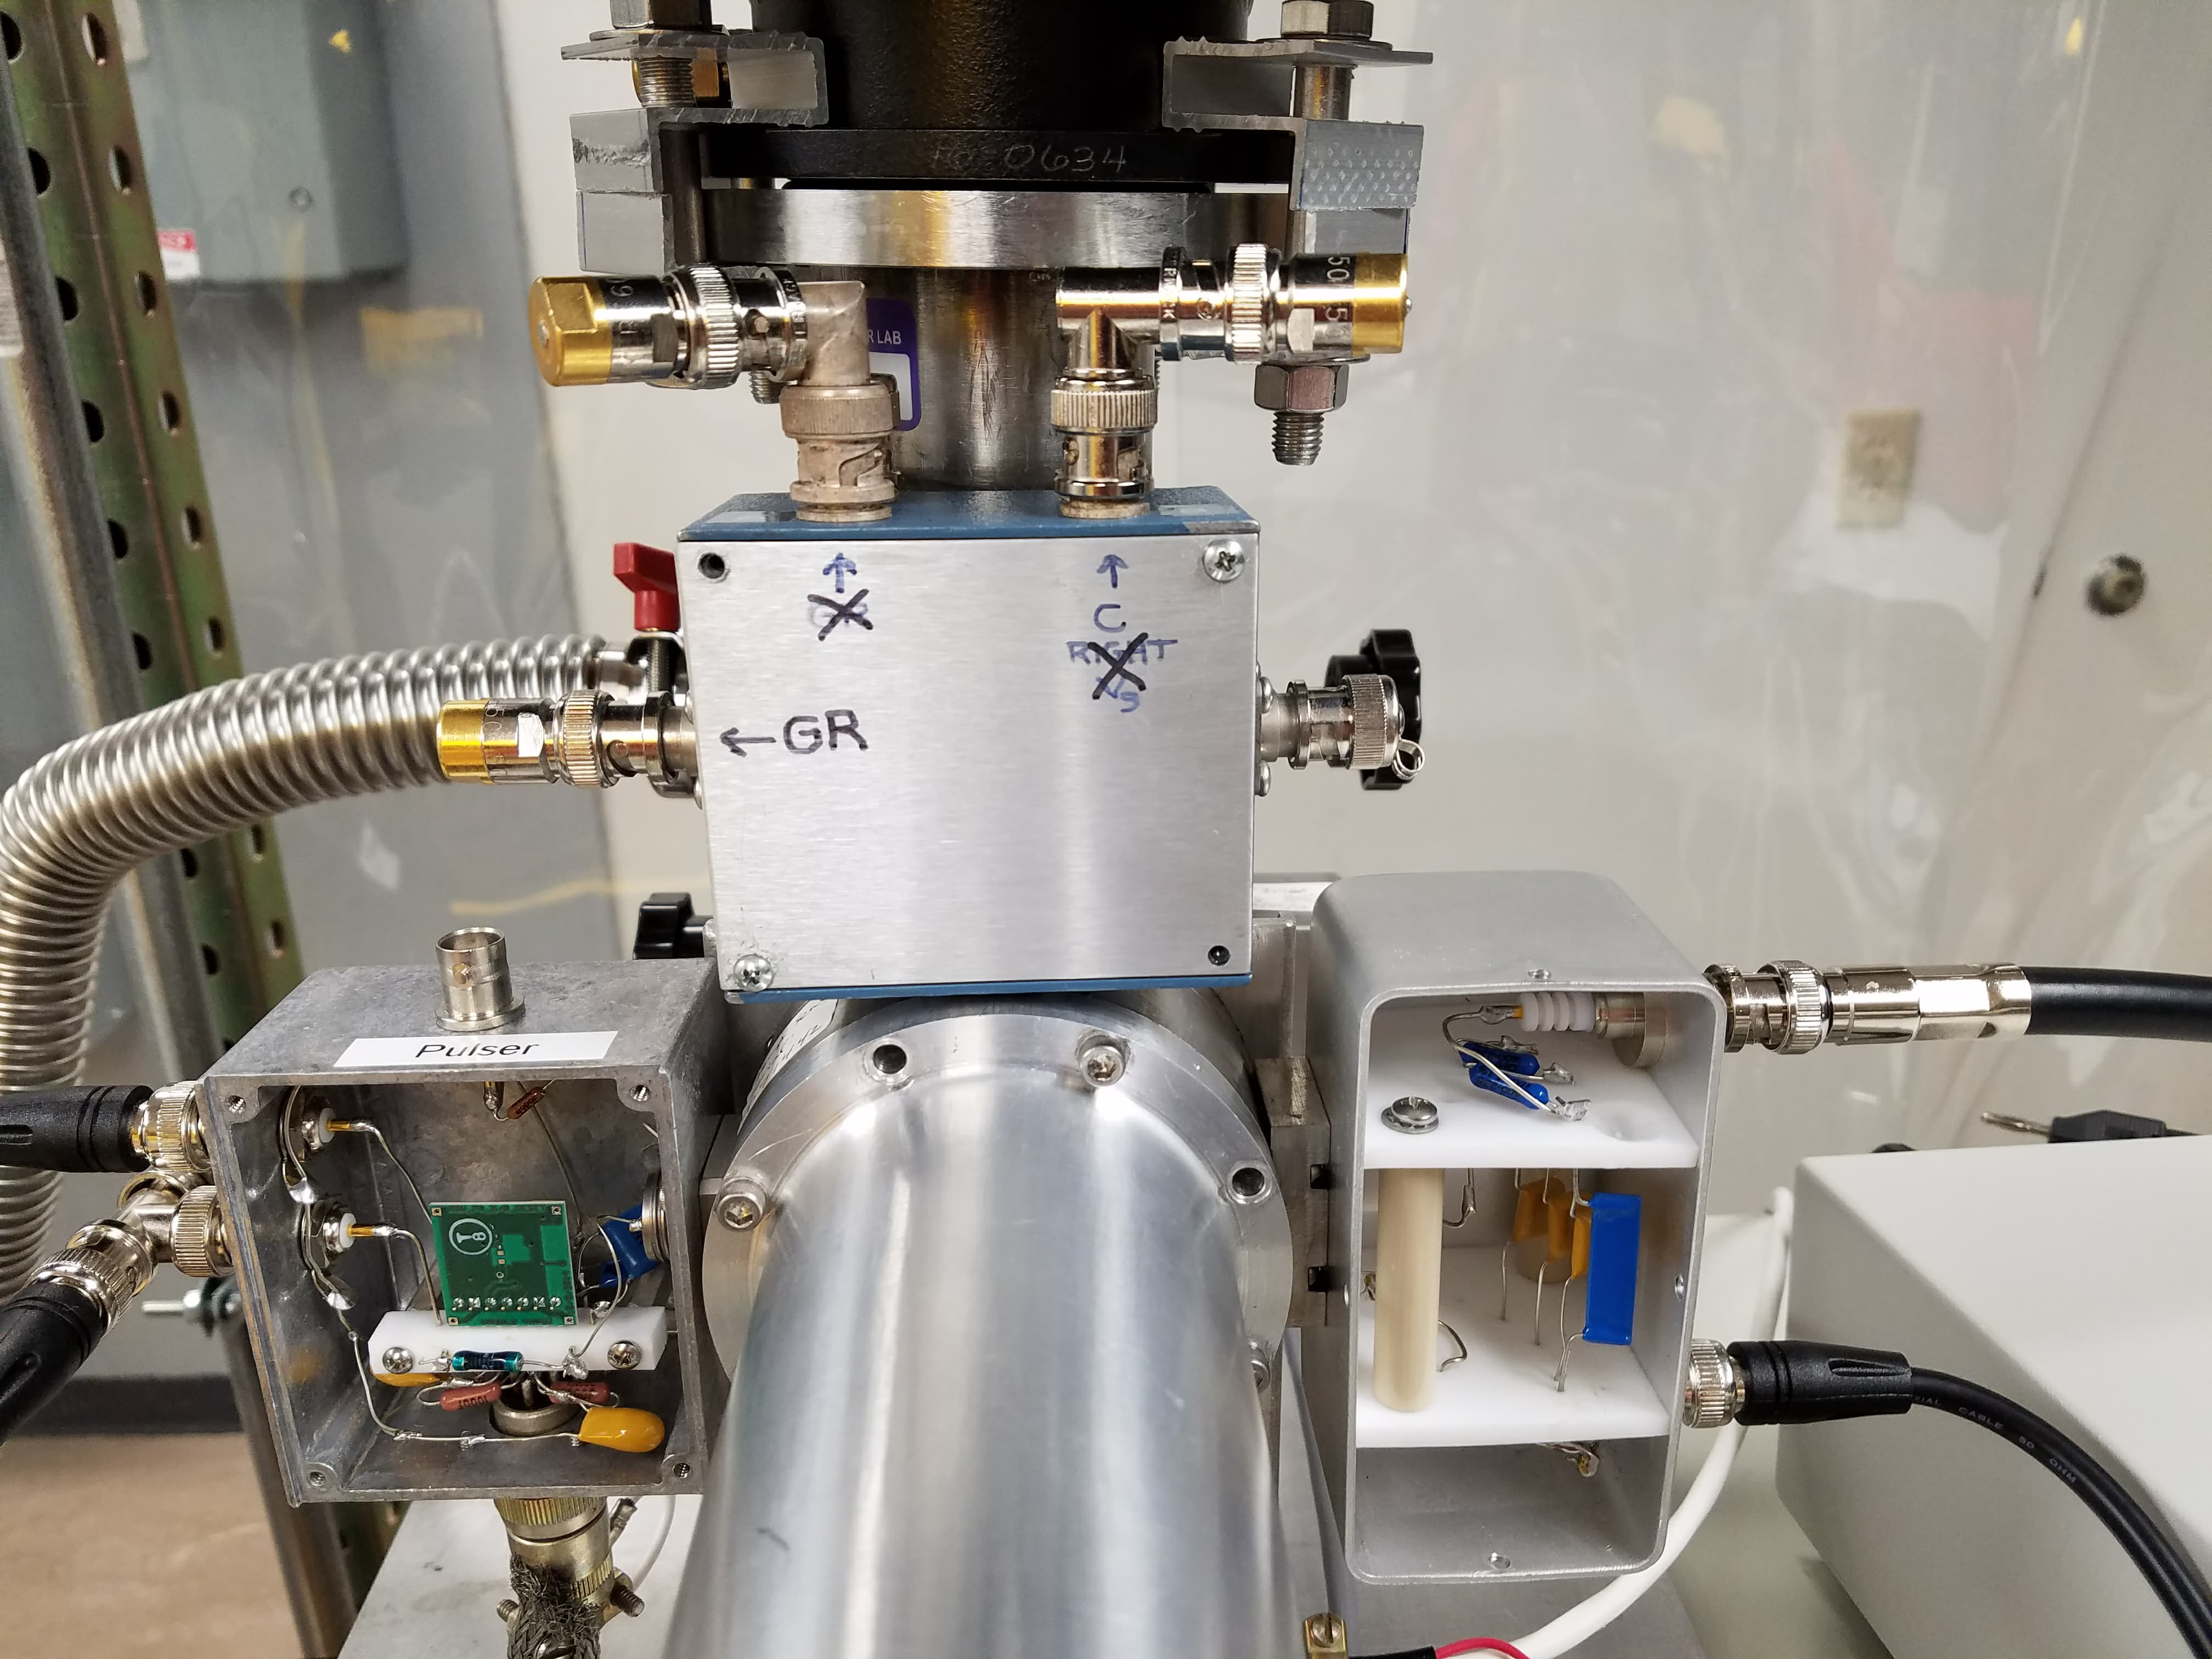
\includegraphics[width=0.7\textwidth]{inputs}
\caption{Zoomed in view of the electrical inputs and circuitry}
\label{fig:inputs}
\end{figure}

\begin{figure}[htpb]
\centering
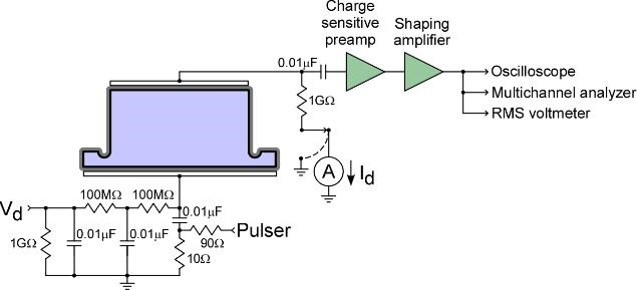
\includegraphics[width=\textwidth]{outline}
\caption{Simple circuit diagram of the germanium detector electronics}
\label{fig:outline}
\end{figure}

\begin{figure}[htpb]
\centering
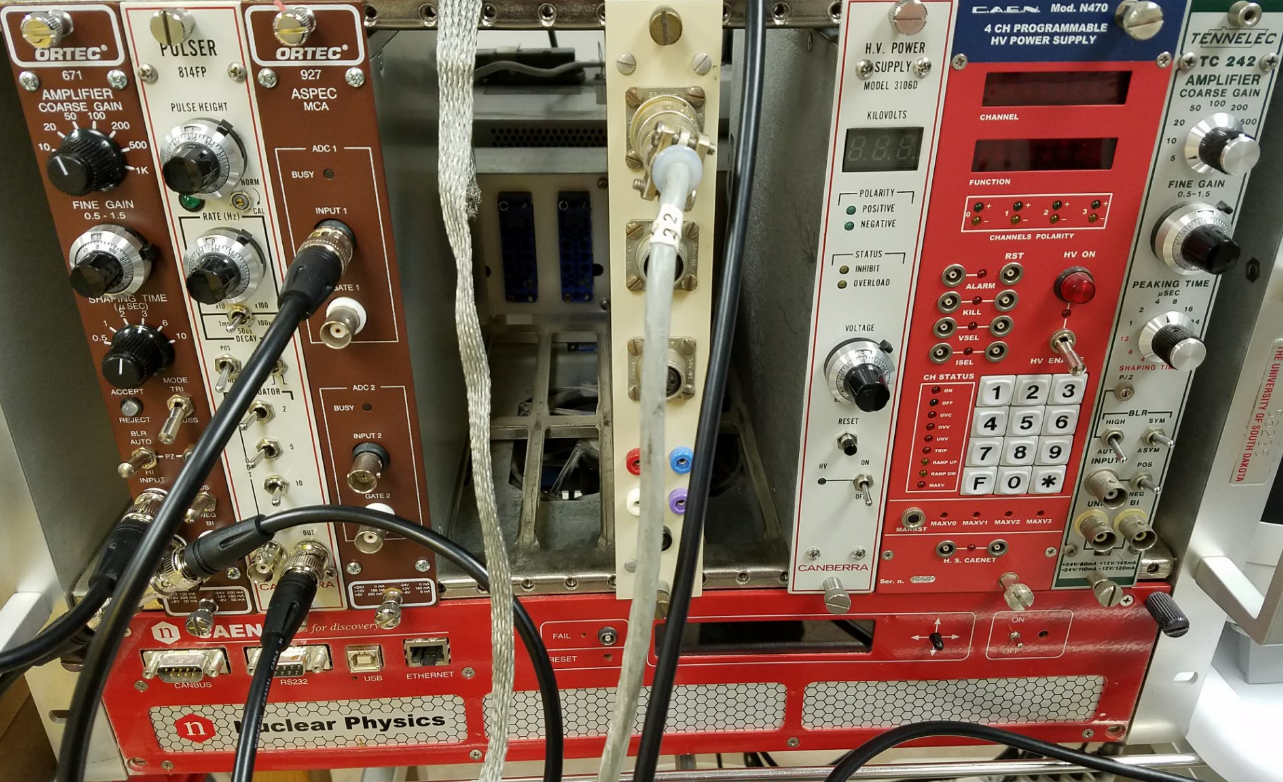
\includegraphics[width=\textwidth]{crate}
\caption{The electronics crate used in detector characterization}
\label{fig:crate}
\end{figure}

\begin{figure}[htpb]
\centering
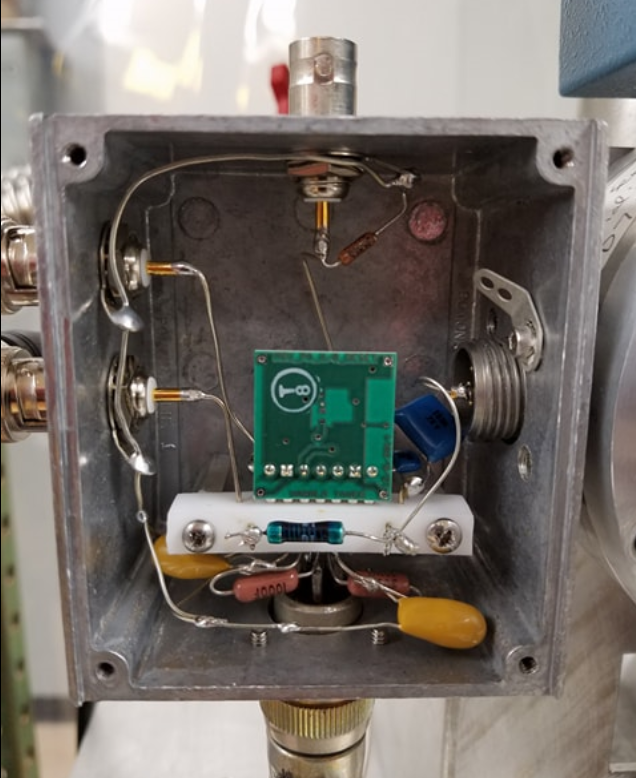
\includegraphics[width=0.7\textwidth]{left-ear}
\caption{Circuit box housing the preamplifier and leakage current assembly}
\label{fig:left-ear}
\end{figure}

\begin{figure}[htpb]
\centering
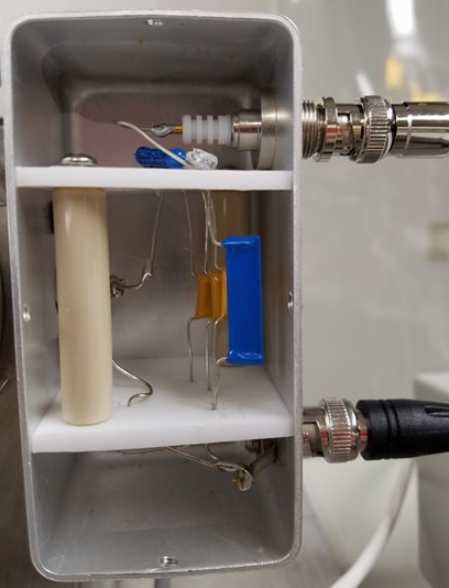
\includegraphics[width=0.7\textwidth]{right-ear}
\caption{Circuit box housing voltage and pulser input along with a high voltage filter}
\label{fig:right-ear}
\end{figure}

\begin{figure}[htpb]
\centering
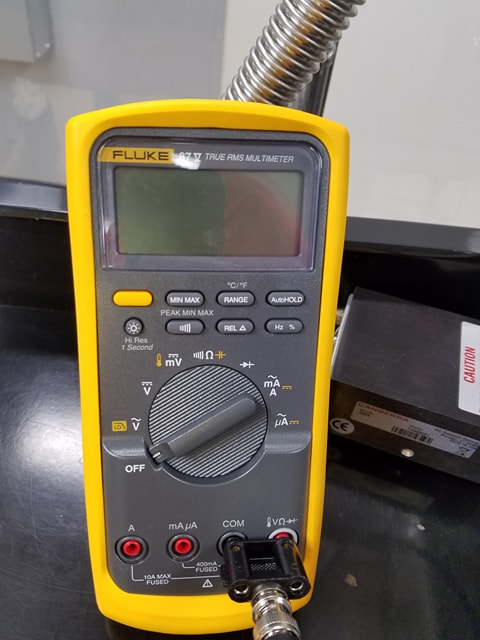
\includegraphics[width=0.7\textwidth]{multimeter}
\caption{Multimeter used to measure leakage current}
\label{fig:multimeter}
\end{figure}

\begin{figure}[htpb]
\centering
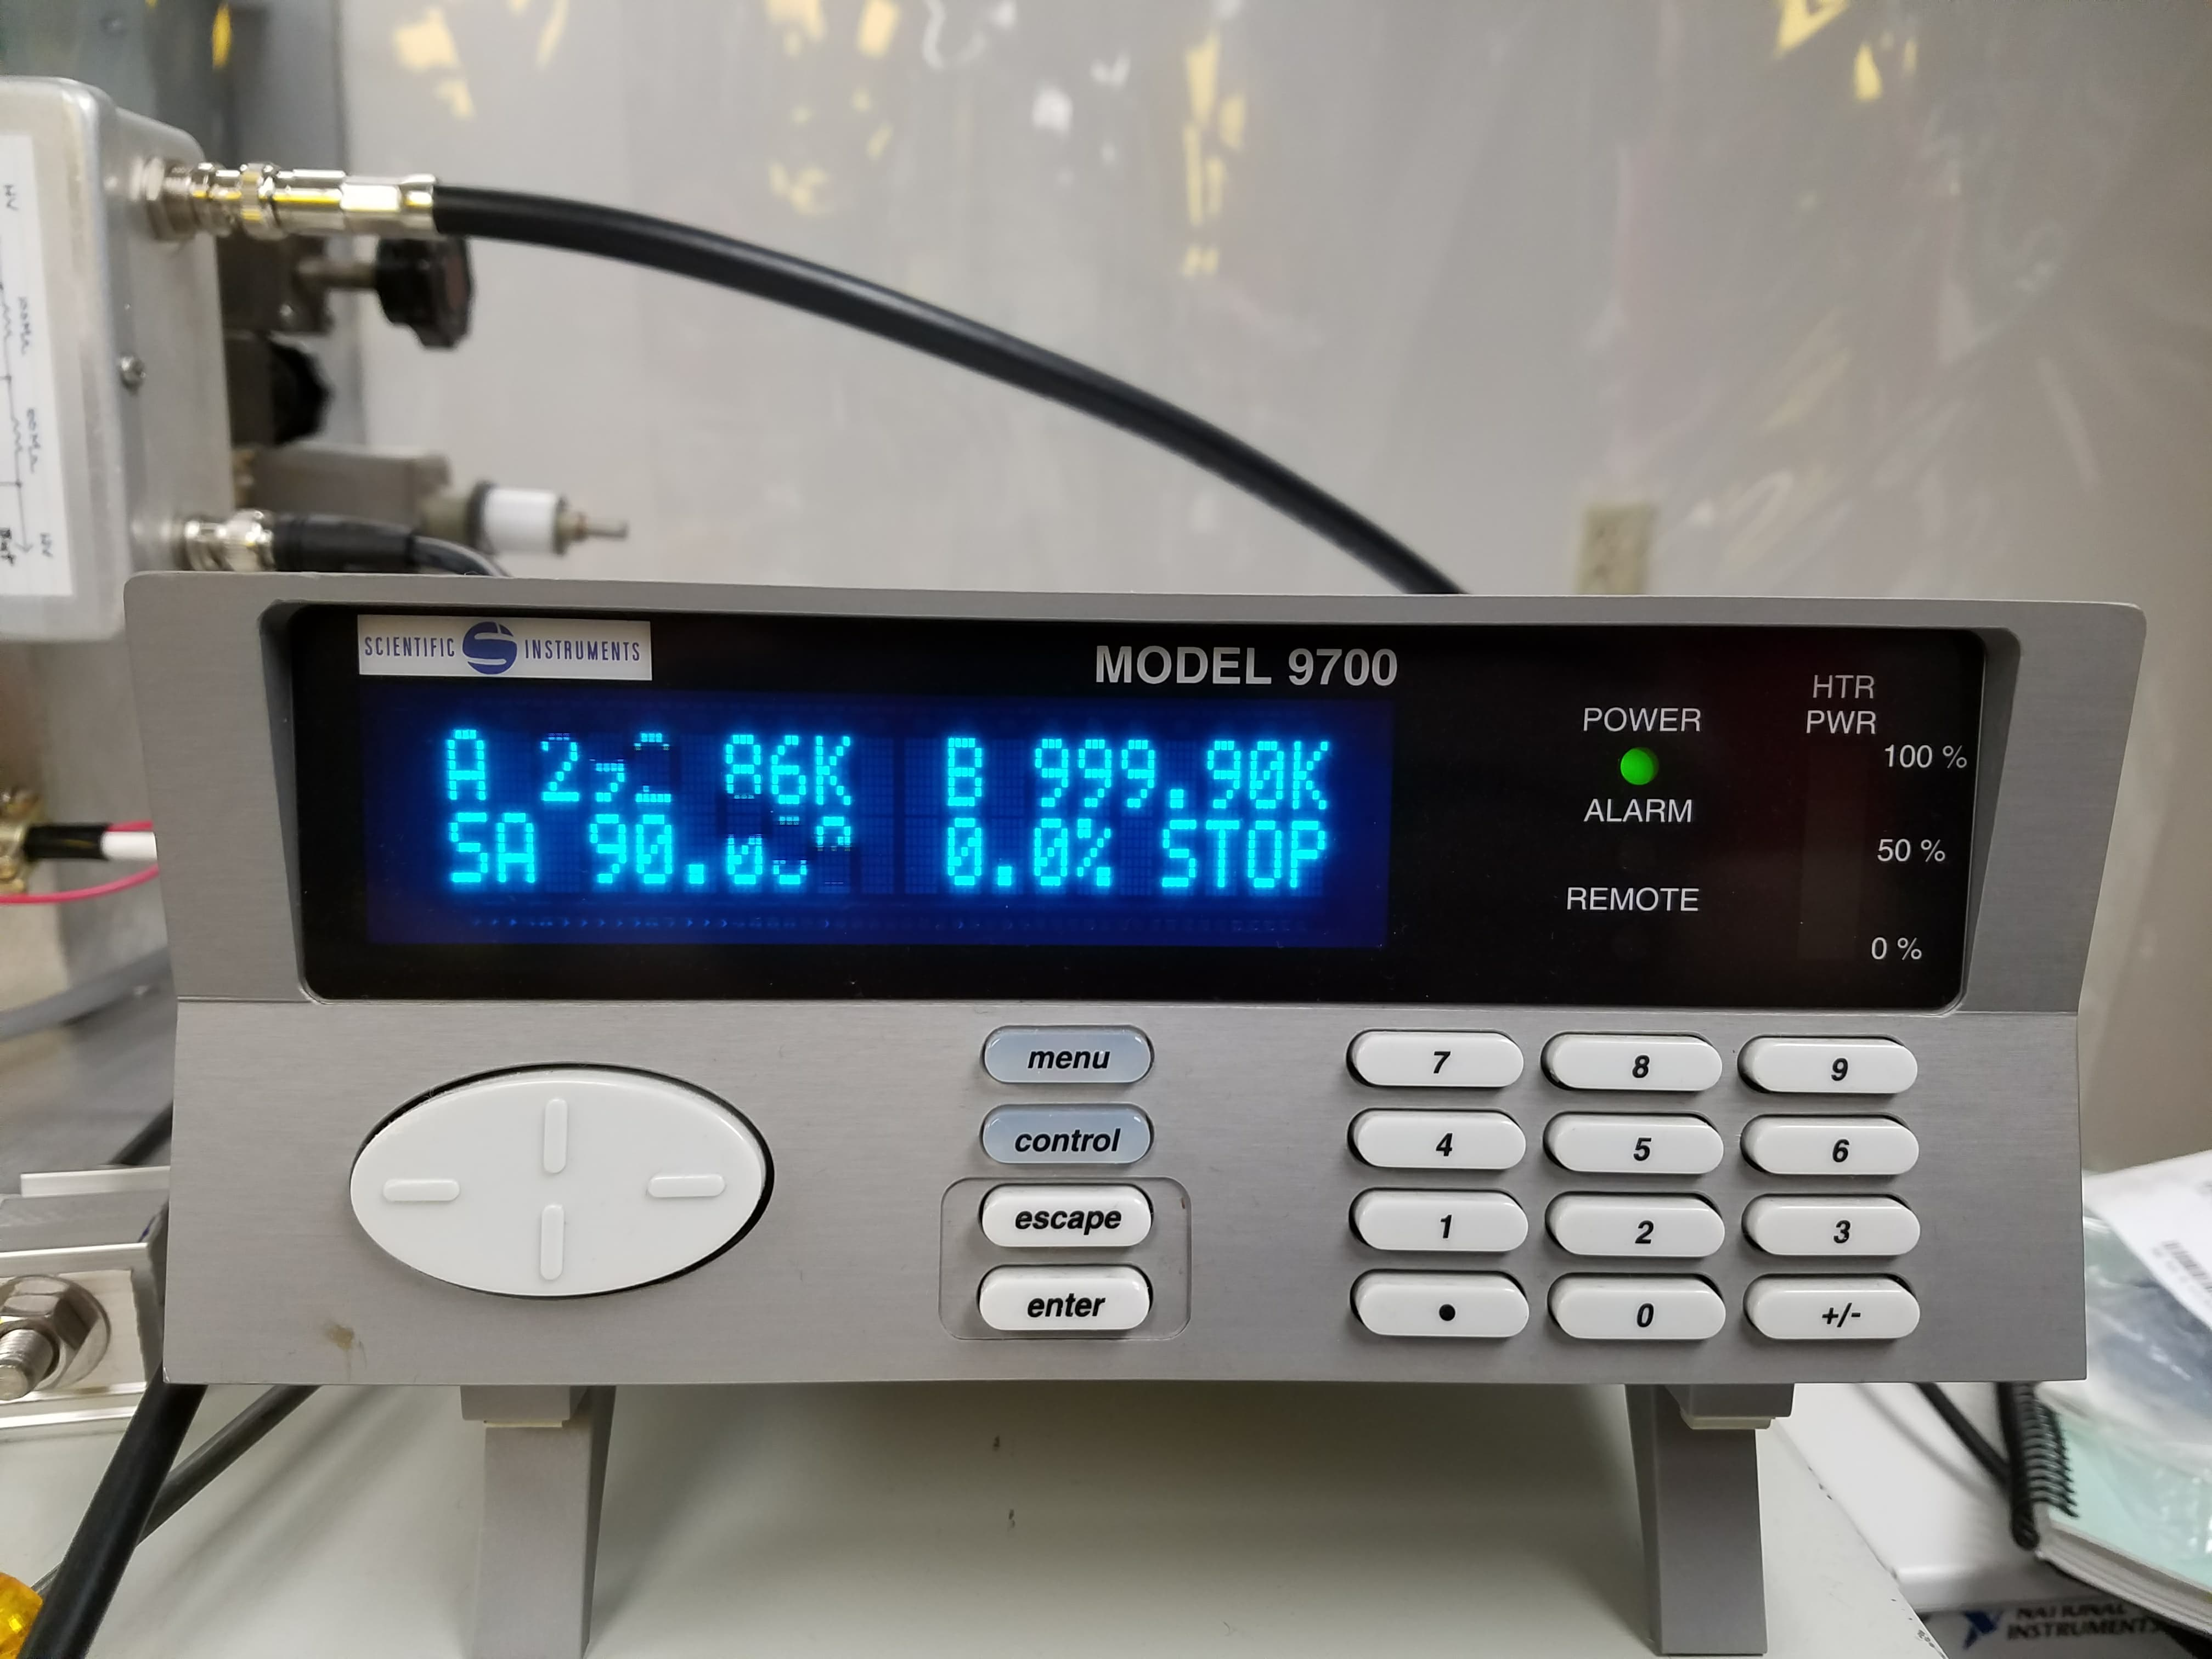
\includegraphics[width=\textwidth]{temp-sens}
\caption{Temperature monitoring and control system with heater}
\label{fig:temp-sens}
\end{figure}

\begin{figure}[htpb]
\centering
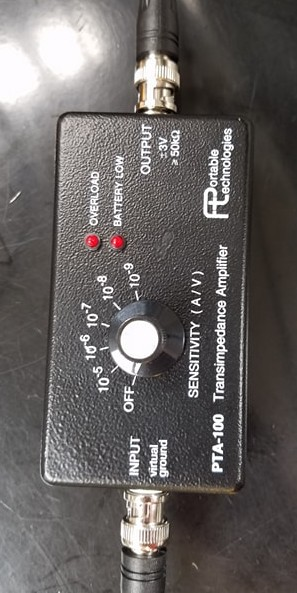
\includegraphics[width=0.5\textwidth]{transimpedence}
\caption{Device for converting low current to voltage}
\label{fig:transimpedence}
\end{figure}


%%%%%%%%%%%%%%%%
% Chapter 7
%%%%%%%%%%%%%%%%

\chapter{Conclusion}


%%%%%%%%%%%%%%%%
% Chapter 8
%%%%%%%%%%%%%%%%

\chapter{Conclusion}


%%%%%%%%%%%%%%%%
% Appendices
%%%%%%%%%%%%%%%%

\begin{appendices}

%Some Table of Contents entry formatting
\addtocontents{toc}{\protect\renewcommand{\protect\cftchappresnum}{\appendixname\space}}
\addtocontents{toc}{\protect\renewcommand{\protect\cftchapnumwidth}{6em}}

%Begin individual appendices, separated as chapters

\chapter{Experimental Equipment}
Lorem ipsum dolor sit amet, consectetur adipiscing elit, sed do eiusmod tempor incididunt ut labore et dolore magna aliqua. Ut enim ad minim veniam, quis nostrud exercitation ullamco laboris nisi ut aliquip ex ea commodo consequat. Duis aute irure dolor in reprehenderit in voluptate velit esse cillum dolore eu fugiat nulla pariatur. Excepteur sint occaecat cupidatat non proident, sunt in culpa qui officia deserunt mollit anim id est laborum.

\begin{sidewaysfigure}
\includegraphics[width=\textwidth]{control-screen}
\caption{These are the four settings screens and translations from the diamond saw controller.}
\label{fig:control-screen}
\end{sidewaysfigure}
\chapter{Data Processing}
Lorem ipsum dolor sit amet, consectetur adipiscing elit, sed do eiusmod tempor incididunt ut labore et dolore magna aliqua. Ut enim ad minim veniam, quis nostrud exercitation ullamco laboris nisi ut aliquip ex ea commodo consequat. Duis aute irure dolor in reprehenderit in voluptate velit esse cillum dolore eu fugiat nulla pariatur. Excepteur sint occaecat cupidatat non proident, sunt in culpa qui officia deserunt mollit anim id est laborum.

\end{appendices}

%}}}
%%%%%%%%%%%%%%%%%%%%%%

%%%%%%%%%%%%%%%%
% References
%%%%%%%%%%%%%%%%

\begin{singlespace}  % use single-line spacing for multi-line text within a single reference
	\setlength\bibitemsep{\baselineskip}  %manually set separataion betwen items in bibliography to double space
	\printbibliography[title={References}]
\end{singlespace}

\addcontentsline{toc}{chapter}{References}  %add References section to Table of Contents



\end{document}
